
% VLDB template version of 2020-08-03 enhances the ACM template, version 1.7.0:
% https://www.acm.org/publications/proceedings-template
% The ACM Latex guide provides further information about the ACM template

\documentclass[sigconf, nonacm]{acmart}

% \usepackage{cite}
% \usepackage{amsmath,amssymb,amsfonts}
\usepackage{algorithm2e}
\usepackage{graphicx}
\usepackage{textcomp}
\usepackage{subcaption}

% %%%%%%%%%%%---My Packages-----%%%%%%
% \usepackage{fancyhdr}
% \usepackage[normalem]{ulem}
% \usepackage[hyphens]{url}
% \usepackage[sort,nocompress]{cite}
% \def\baselinestretch{0.9}
% Always include hyperref last
% \usepackage[bookmarks=true,breaklinks=true,letterpaper=true,colorlinks,linkcolor=black,citecolor=blue,urlcolor=black]{hyperref}
\usepackage[binary-units=true]{siunitx}
% \sisetup{per-mode=symbol,per-symbol = /}
% \usepackage{mathtools}
\usepackage{booktabs}
% \usepackage[dvipsnames]{xcolor}
\usepackage{enumitem}
\usepackage[skip=2pt]{caption}
%%%%%%%%%%%%%%%%%%%%%%%%%%%%%%%%%%%%
%%%%%%%%%%%%---Math operators-----%%%%%%%%%%%
\DeclareMathOperator{\PR}{PR}
\DeclareMathOperator{\PRprime}{PR^\prime}
\DeclareMathOperator{\PRnext}{PR_{next}}
\DeclareMathOperator{\inNeighbors}{inNeighbors}
\DeclareMathOperator{\outDegree}{outDegree}
\DeclareMathOperator{\divClause}{divClause}
\DeclareMathOperator{\divClauseMin}{divClause_{min}}
\DeclareMathOperator{\divClauseMax}{divClause_{max}}
\DeclareMathOperator{\clampRange}{clamp_{range}}
\DeclareMathOperator{\rangMin}{Range_{min}}
\DeclareMathOperator{\rangMax}{Range_{max}}
\DeclareMathOperator*{\Sum}{\mathlarger{\sum}}
\DeclareMathOperator*{\SSum}{\mathlarger{\mathlarger{\mathlarger{\sum}}}}
%%%%%%%%%%%%%%%%%%%%%%%%%%%%%%%%%%%%%%%%%%%%%

%% The following content must be adapted for the final version
% paper-specific
\newcommand\vldbdoi{XX.XX/XXX.XX}
\newcommand\vldbpages{XXX-XXX}
% issue-specific
\newcommand\vldbvolume{14}
\newcommand\vldbissue{1}
\newcommand\vldbyear{2020}
% should be fine as it is
\newcommand\vldbauthors{\authors}
\newcommand\vldbtitle{\shorttitle} 
% leave empty if no availability url should be set
\newcommand\vldbavailabilityurl{https://github.com/atmughrabi/GraphBrew}
% whether page numbers should be shown or not, use 'plain' for review versions, 'empty' for camera ready
\newcommand\vldbpagestyle{plain} 

\begin{document}
\title{GraphBrew: Multilayered Graph Reordering for Accelerated Graph Processing}

%%
%% The "author" command and its associated commands are used to define the authors and their affiliations.
\author{Abdullah T. Mughrabi}
\affiliation{%
  \institution{Department of Computer Science, University of Virginia}
  \city{Charlottesville}
  \state{Virginia}
  \country{USA}
}
\email{atmughra@virginia.edu}
\email{atmughra@alumni.ncsu.edu}

\author{Mohannad M. Ibrahim}
\affiliation{%
  \institution{Department of Electrical and Computer Engineering, North Carolina State University}
  \city{Raleigh}
  \state{North Carolina}
  \country{USA}
}
\email{mmibrah2@alumni.ncsu.edu}

\author{Morteza Baradaran}
\affiliation{%
  \institution{Department of Computer Science, University of Virginia}
  \city{Charlottesville}
  \state{Virginia}
  \country{USA}
}
\email{rgq5aw@virginia.edu}

\author{Beenish Gul}
\affiliation{%
  \institution{Department of Computer Science, University of Virginia}
  \city{Charlottesville}
  \state{Virginia}
  \country{USA}
}
\email{bg9qq@virginia.edu}


\author{Gregory T. Byrd}
\affiliation{%
  \institution{Department of Electrical and Computer Engineering, North Carolina State University}
  \city{Raleigh}
  \state{North Carolina}
  \country{USA}
}
\email{gbyrd@ncsu.edu}

\author{Kevin Skadron}
\affiliation{%
  \institution{Department of Computer Science, University of Virginia}
  \city{Charlottesville}
  \state{Virginia}
  \country{USA}
}
\email{skadron@virginia.edu}
%%
%% The abstract is a short summary of the work to be presented in the
%% article.
\begin{abstract}
Graph algorithms exhibit random fine-grain memory access patterns that cause low temporal and spatial cache locality. One widely used strategy to reduce the high cache miss rate in graph processing is to reorder the graph structure labels by utilizing the input graph community structures and real-world characteristics. Although graph reordering improves algorithm execution time with better caching, it adds high costs to end-to-end graph processing execution time. This overhead motivates the need for lightweight graph reordering techniques that incorporate fewer graph structure features, achieving suboptimal graph caching but better end-to-end performance.

In this paper, we first demonstrate how specific lightweight reordering techniques fail to deliver a comprehensive solution for various graph algorithms and graph input structures compared to Gorder, a sophisticated graph reordering algorithm with high overhead. We then introduce GraphBrew, a scheme that incorporates multilayered lightweight reordering techniques. GraphBrew Combines various features from the input graph while utilizing multiple lightweight reordering stages---thus maintaining low reordering overhead while delivering high cache performance. With GraphBrew, we achieve up to 6x speedup graph-reordering execution over Gorder, while maintaining similar graph algorithm performance.
\end{abstract}

\maketitle

%%% do not modify the following VLDB block %%
%%% VLDB block start %%%
\pagestyle{\vldbpagestyle}
\begingroup\small\noindent\raggedright\textbf{PVLDB Reference Format:}\\
\vldbauthors. \vldbtitle. PVLDB, \vldbvolume(\vldbissue): \vldbpages, \vldbyear.\\
\href{https://doi.org/\vldbdoi}{doi:\vldbdoi}
\endgroup
\begingroup
\renewcommand\thefootnote{}\footnote{\noindent
This work is licensed under the Creative Commons BY-NC-ND 4.0 International License. Visit \url{https://creativecommons.org/licenses/by-nc-nd/4.0/} to view a copy of this license. For any use beyond those covered by this license, obtain permission by emailing \href{mailto:info@vldb.org}{info@vldb.org}. Copyright is held by the owner/author(s). Publication rights licensed to the VLDB Endowment. \\
\raggedright Proceedings of the VLDB Endowment, Vol. \vldbvolume, No. \vldbissue\ %
ISSN 2150-8097. \\
\href{https://doi.org/\vldbdoi}{doi:\vldbdoi} \\
}\addtocounter{footnote}{-1}\endgroup
%%% VLDB block end %%%

%%% do not modify the following VLDB block %%
%%% VLDB block start %%%
\ifdefempty{\vldbavailabilityurl}{}{
\vspace{.3cm}
\begingroup\small\noindent\raggedright\textbf{PVLDB Artifact Availability:}\\
The source code, data, and/or other artifacts have been made available at \url{\vldbavailabilityurl}.
\endgroup
}
%%% VLDB block end %%%


\section{Introduction}
Graph analytics are prevalent in many domains, playing an essential role in social networks, biomedical sciences, and graph neural networks (GNNs) \cite{ang_introducing_2010,lee_extrav_2017,zhou_graph_2019}. The broad adoption of graph processing is due to graph data structures' presenting a powerful abstraction that streamlines graph algorithm implementations. In conjunction with graph analytics becoming everywhere, performance challenges arise from a high ratio of random fine-grain memory accesses over large data sets. Such accesses overwhelm the target system bandwidth while causing high cache miss rates \cite{lumsdaine_challenges_2007,beamer_locality_2015,beamer_reducing_2017,wei_speedup_2016}.

\begin{figure}[t]
  \centering
  
\includegraphics[width=\linewidth]{paperFigures/Fig3}
  \caption{Graph representation in CSR format, accessing vertex data is non sequential and fine-grained, with high cache miss rate.}
  \label{fig:fig3}
\end{figure}

Fig.~\ref{fig:fig3} illustrates a conventional graph processing approach in shared memory systems, known as a vertex-centric \cite{mccune_thinking_2015} or a Gather-Apply-Scatter (GAS) model. As shown in Algorithm~\ref{algo:fig2}, the vertex-centric approach employs a Compressed Sparse Row (CSR) matrix data structure to represent the graph in memory for easy neighbor access. Visiting the neighbors for each vertex in a streamlined manner might seem intuitive with the GAS model. However, the scattering of neighbor IDs for each visited vertex generates irregular memory access patterns, leading to low spatial and temporal locality with a high cache miss rate.

\begin{algorithm}[b]
	\SetAlgoLined
	\leftline{
\includegraphics[width=0.7\linewidth]{paperFigures/Fig2}}
	\caption{Graph traversal, with CSR structure.}
	\label{algo:fig2}
\end{algorithm}

One key characteristic of graph vertices is their \emph{power-law} or skewed degree distribution \cite{barabasi_scale-free_2009,zhang_making_2017,balaji_when_2018,faloutsos_power-law_1999,beamer_gap_2017,zhang_optimizing_2016}. \emph{Power-law} graphs represent a graph topology with a small percentage of vertices holding the majority of connections. Such graphs are prevalent in various applications like social networks and are often characterized by \emph{power-law} distributions and noted as \emph{scale-free} or \emph{natural} graphs.
The internal labeling of vertices can also contribute to a bottleneck during graph traversal. For instance, traversing or exploring a graph often starts with a vertex-centric graph algorithm propagating through a source vertex and then visiting its neighboring vertices, as shown in Algorithm ~\ref{algo:fig2}. The algorithm traversal performance depends on many factors. However, one main factor affecting the cache and overall memory bandwidth performance is how the data accessed within and across graph community clusters are spatially and temporally coalesced.

Previous research has demonstrated cache optimizing techniques for better bandwidth utilization through reordering vertex IDs \cite{arai_rabbit_2016,balaji_when_2018,balaji_combining_2019,faldu_closer_2020,wei_speedup_2016}. Such techniques exploit graph skewness and clustering to improve the source's vertex caching with its neighboring vertices across the graph vertex data arrays. The main issue of using reordering techniques is how sophisticated or lightweight they are. Fig.~\ref{fig:fig1} shows an approximation of the end-to-end performance with different reordering techniques. Generally, more sophisticated analysis techniques lead to better cache locality and performance, but the cost of performing the analysis leads to higher end-to-end latency. Pre-processing time \cite{malicevic_everything_2017}, which includes reading the graph edge-list from the file and building the CSR structure as demonstrated in Fig.~\ref{fig:fig3}, is increased with a reorder step. Consequently, the higher overhead of sophisticated reordering techniques degrades pre-processing performance. Higher pre-processing latency may not be overcome by improved cache performance, leading to longer end-to-end latency.

This study introduces GraphBrew, a novel multilevel lightweight reordering scheme. GraphBrew adopts multiple layers of lightweight reordering routines, optimizing certain features in the graph structure to maintain the low overhead of lightweight reordering while obtaining the cache performance of sophisticated reordering techniques.  The first layer will incorporate Leiden Community detection \cite{traag_louvain_2019}, a hierarchical community-based ordering, achieving high locality while mapping vertices according to CPU cache hierarchies and graph community structures. The second layer applies Degree Based Grouping (DBG) \cite{faldu_closer_2020}, which groups hot and cold vertices by their degrees while maintaining the optimized, community-based ordering inside the graph. Consequently, the ordering and cache performance quality is on par with more sophisticated techniques like state-of-the-art Gorder \cite{wei_speedup_2016}.

Our main contributions in this paper are summarized as follows:
\begin{itemize}[topsep=2pt,itemsep=2pt,wide]
\item We evaluate the caching performance for the state of the art reordering techniques on a selection of graph algorithms and demonstrate how the caching performance depends on the graph algorithm and graph topology with the reordering method used.
\item We outline the design of GraphBrew, a novel multilayered reordering scheme for achieving high end-to-end performance while obtaining the caching quality of a state of the art graph reordering algorithms.
\item We evaluate GraphBrew across various graph structures and graph algorithms and contrast it against DBG, Rabbit Order, and Gorder.
\item We present results showing better pre-processing time and graph algorithm performance than Gorder. Furthermore, more speedups in end-to-end performance against DBG and Rabbit Order.
\end{itemize}

 \begin{figure}[b]
  \centering
  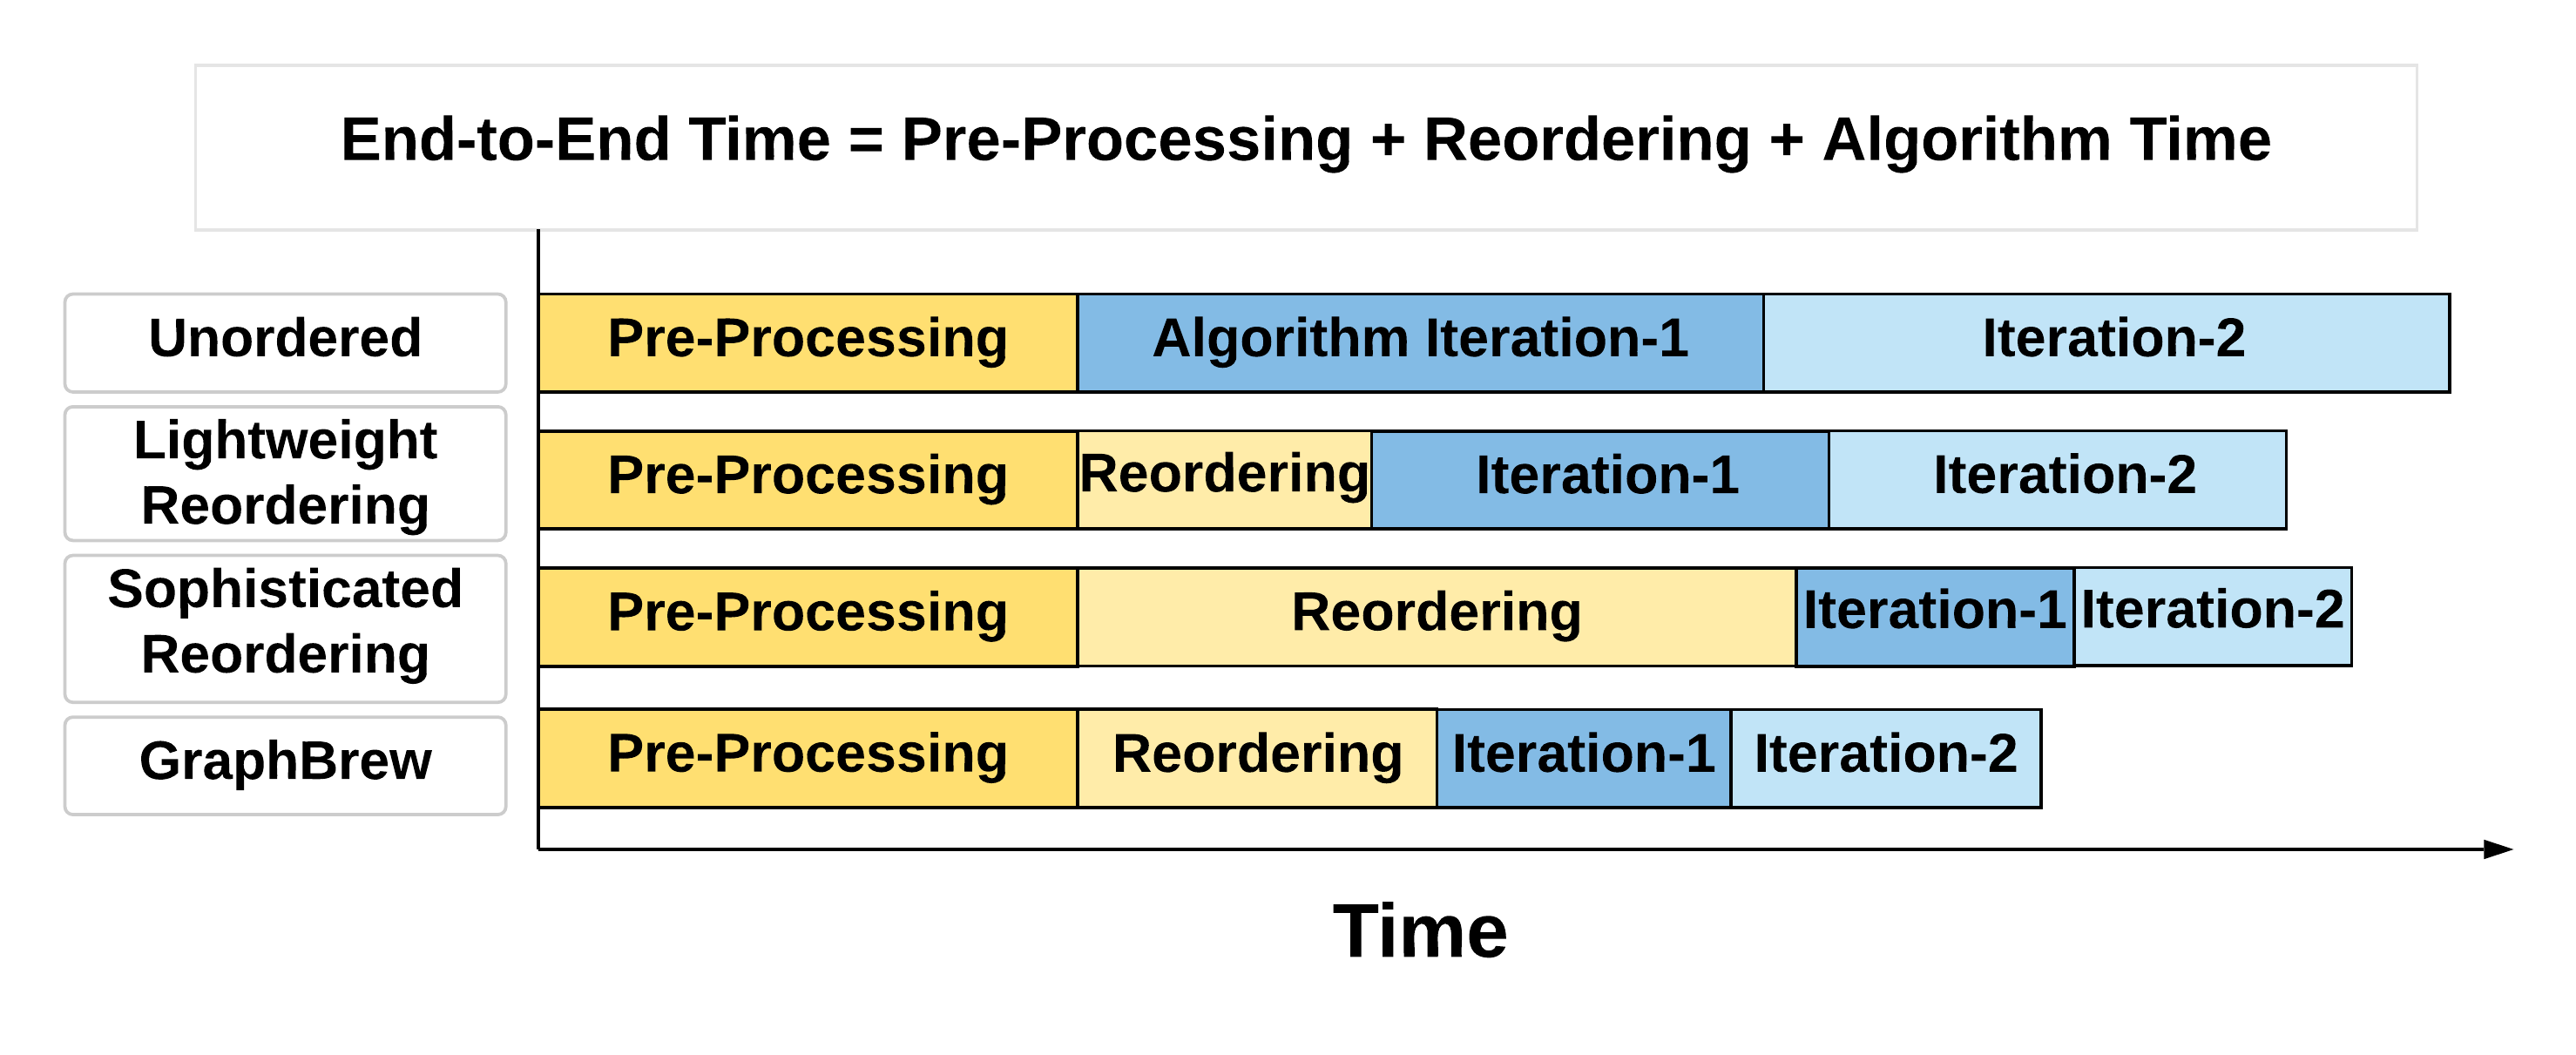
\includegraphics[width=\linewidth]{paperFigures/Fig1c}
  \caption{Graph Pre-processing overhead trade-offs. Adding reordering might benefit the graph algorithm performance, but harms end-to-end execution time.}
  \label{fig:fig1}
\end{figure}

\section{Background and Motivation}

\subsection{Graph Algorithms Taxonomy}
Graph algorithm access patterns usually fall into a few well-known categories. These categories are essential to understand why graph algorithm performance suffers from irregular memory access patterns with a high cache miss ratio while processing the input graph structure. There is a growing body of literature \cite{beamer_direction-optimizing_2012, besta_push_2017} that recognizes these behavioral patterns in conjunction with utilizing vertex-centric graph algorithms with CSR data structures as listed below:

\begin{itemize}[topsep=2pt,itemsep=2pt,wide]
\item \textbf{Iterative:} An iterative graph algorithm processes all the graph vertices in each iteration until reaching a convergence criterion. This behavior often requires a cache that fits the whole graph dataset for fewer capacity misses and less thrashing. Iterative algorithms can benefit from reordering, with each community \cite{arai_rabbit_2016} within the graph labeled closely together for better scheduling when looping within each iteration and reading the graph data arrays \cite{mukkara_exploiting_2018}. Good examples of iterative algorithms are PageRank (PR) and Sparse Matrix-Vector Multiplication (SpMV).
\item \textbf{Traversal:} A traversing algorithm typically starts from a source vertex and propagates through the vertex neighbors in a frontier manner through the graph. Each traversal activates the neighboring vertices in the frontier. Such behavior often requires caching the active vertices set within a graph community on frontier traversal bases. Furthermore, there is a high probability of visiting high degree vertices in the graph within each traversal, giving the incentive to reorder according to the graph degree skewness.  Good examples of traversal algorithms are Breadth-First Search (BFS), Single Source Shortest Path (SSSP), and Connected Components (CC).
\item \textbf{Pull-Based:} The pull-based approach describes data propagation between vertices in the processed graph. With a pull-based graph algorithm, the processed vertex gathers data from neighboring vertices while updating itself. This technique is effective in parallel implementation of graph algorithms where each core is scheduled a single vertex in parallel, eliminating the need for locks \cite{besta_push_2017}. Relabeling graph vertices in pull-based algorithms requires grouping hot (frequently-used) vertices based on their out-degree for better caching. For instance, vertex with higher out-degree have a higher probability of being read by the other vertices giving the incentive of retaining them in the cache together longer.
\item \textbf{Push-Based:} The push-based strategy behaves as a counterpart to the pull-based approach for data propagation between vertices \cite{besta_push_2017} . The vertex pushes or propagates the data to neighboring vertices in the input graph, updating the neighboring vertices. Push-based graph algorithms often need locks to prevent race conditions when two vertices share the same neighbor and push data simultaneously. Although the push-based method usually creates locking overhead, hence hurting performance, in some cases it simplifies the graph algorithm implementation by eliminating the need for an inverse graph memory overhead. For example, data-driven PageRank (PR) \cite{whang_scalable_2015} graph algorithms use a push-based approach to propagating data, leading to faster conversion for less iteration. Finally, when it comes to relabeling vertices, grouping hot vertices with high in-degree achieves the best performance. The in-degree groupings give a higher probability for hot vertices to remain in the cache while being updated frequently by a single core. 
\end{itemize}

\subsection{Graph Algorithms Suite}

This paper introduces XXX, an open-source graph processing benchmark suite built with OpenMP. This suite provides an end-to-end evaluation infrastructure, including the pre-processing, reordering, and graph algorithms steps. Furthermore, it adopts a modular implementation for a more straightforward evaluation of each step, unlike other benchmark suites. The framework also re-implements and matches the performance of other popular benchmark suites \cite{beamer_gap_2017,shun_ligra_2013} to maintain a consistent frame of reference when comparing to other bodies of work. XXX is available at:  \url{https://github.com/XXX/XXX}.

\begin{itemize}[topsep=2pt,itemsep=2pt,wide]
\item \textbf{Breadth First Search (BFS) (Iterative, Push): }
BFS is an essential step in many graph algorithms. It is widely used as a building block for other graph algorithms such as  Connected Components and Single-Source Shortest Path \cite{beamer_direction-optimizing_2012}.
This traversal-based graph algorithm starts from a source or \emph{root} vertex, and its frontier expands outwards at each algorithm step. At each iteration, all vertices at the same depth are visited before moving to the next depth. A conventional BFS approach that yields a BFS tree from a graph structure consists of checking all neighbors of a source vertex $v$ to see if any are unvisited. Each unvisited neighbor is then marked as visited and added to the frontier as it expands \cite{beamer_gap_2017,besta_push_2017}.

%d

\item \textbf{PageRank (PR) (Iterative, Pull): }
PageRank \cite{page_pagerank_1999,brin_anatomy_1998,bianchini_inside_2005,beamer_gap_2017} is an example of an iterative graph algorithm. At each iteration, the algorithm traverses the graph vertices assigning a popularity score (rank) to each vertex. A vertex's rank is essentially derived from the ranks of its incoming edges (in-neighbors). The algorithm iterates until the ranks converge within a specified error margin. PageRank's equation is outlined as follows:
\begin{equation}\label{eqn:pr}
	{
		\PR(v) := \text{\footnotesize $  \alpha \left ( \frac{1}{N} \right ) +(1-\alpha) \Sum_{u\in \inNeighbors(v)} \frac{\PR(u)}{\outDegree(u)} $}
	}
\end{equation} %
where ${N}$ is the total number of vertices in the graph. The random jump \emph{teleportation} factor $\alpha$ and the damping factor $(1-\alpha)$, help PR reach convergence. In layman's terms, \eqref{eqn:pr} defines the pagerank of a vertex as the sum of the scaled ranks of its neighboring vertices $(u)$ (in-neighbors), each scaled by its corresponding out-degree.

\item \textbf{Single Source Shortest Path (SSSP) (Iterative, Push): }
The Single-Source Shortest Path (SSSP) algorithm finds the shortest paths between a vertex $v$ and all other vertices in a weighted graph.

The Bellman–Ford algorithm \cite{bellman_routing_1958,ford_jr_network_1956} is one of the major algorithms to solve the SSSP problem. It follows a \emph{relaxation} approach, in which an approximation (overestimate) of the shortest path between the source $v$ and any vertex $u$ is iteratively replaced by better (shorter) ones until the last iteration of the algorithm. 

The algorithm initializes the distance to source $v$ to 0 and to all other destinations to infinity. The algorithm runs for $(n-1)$ iterations, where $n$ is the number of vertices in the graph. At each iteration, the algorithm visits all graph edges. If the distance to a destination can be shortened by taking the edge, the algorithm updates it to the new lower value. At each iteration $i$, the algorithm finds all shortest paths of at most $i$ edges. Since the longest possible path can at most be $(n-1)$ edges away, the algorithm must scan the edges $(n-1)$ times to ensure the shortest path is found for all destinations.

\item \textbf{Sparse Matrix-Vector Multiplication (SpMV) (Iterative, Traversal, Pull): }
SpMV is a broadly used computational kernel in many scientific applications and iterative linear solvers. \ref{eqn:SpMV} shows the general equation for SpMV. Input matrix $A$ is sparse while both vectors $x$ (input) and $y$ (output) are dense.

\begin{equation}\label{eqn:SpMV}
	{
		y=Ax
	}
\end{equation}

For applications requiring multiple runs of SpMV with the same input $A$, the large, irregularly sparse nature of the matrix causes an irregular access pattern and poor cache performance \cite{akbudak_technical_2012}. Hence, storing $A$ using efficient data structures such as Compressed Sparse Row matrix (CSR) can lead to high performance gains.

\item \textbf{Connected Components (CC) (Iterative, Pull): }
This algorithm is usually considered one of the most elementary and commonly used graph algorithms with applications in many fields such as computer vision, spin models in physics, VLSI circuit design, and communication networks \cite{greiner_comparison_1994}.

Consider an undirected graph $G = (V,E)$, where $V$ is the graph vertices (of size $n$) and $E$ is the graph edges (of size $m$). The connected components of $G$ are the sets of vertices such that all vertices in each set are mutually connected (there exists a path between each vertex), and no two vertices from different sets are connected \cite{greiner_comparison_1994}. In particular, we want to label each vertex such that all vertices of a connected component have the same label distinct from that of another connected component and disconnected vertices (vertices of zero degree) should each get their own label \cite{beamer_gap_2017}. There have been many variants of the algorithm and we considered the Shiloach-Vishkin, which is an $O(log n)$ parallel connectivity algorithm with each of its steps taking $O(m)$ \cite{shiloach_ologn_1982}. The algorithm consists of an intermixed application of two main operations: \emph{hooking} and \emph{shortcutting}. Hooking is when one tree is hooked onto another using edges. The trees are also subject to shortcutting that decreases their height using pointer jumping. 
\end{itemize}


\section{GraphBrew}
\subsection{Cache Locality in Graphs}

Fig.~\ref{fig:fig7} showcases how graph algorithm frameworks process the compressed sparse row (CSR) structure, including some of the effects of the vertex label on cache locality. CSR provides a compact and memory-efficient way to process graphs in memory while making it easier to visit the neighbors of the processed vertex. The temporal locality is evident between vertices with shared neighbors; vertices with high degrees have a higher probability of being shared between vertices, so grouping them in a memory region should be beneficial to cache performance. Spatial locality represents vertices grouping within the graph community. For instance, requesting the neighbor data of a processed vertex should touch cache lines spatially. 

\begin{figure}[b]
  \centering
  
\includegraphics[width=\linewidth]{paperFigures/Fig7}
  \caption{Locality and caching in Graph CSR structures.}
  \label{fig:fig7}
\end{figure}

\subsection{Graph Reordering Techniques}

\begin{figure}[t]
  \centering
  
\includegraphics[width=\linewidth]{paperFigures/Fig5}
  \caption{How graph reordering preserves the topology of the graph.}
  \label{fig:fig5}
\end{figure}

Previous studies have shown reordering graphs is an effective method for optimizing  cache performance while accessing the graph data arrays. The central concept behind graph structure reordering is applying new vertex labels which coalesce neighbor vertex data accesses according to their temporal or spatial reuse. As Fig.~\ref{fig:fig5} illustrates, updating vertex IDs for the graph does not affect its structural topology while choosing a sequence of labels based on degree count, community structure, or a more sophisticated model.

\begin{itemize}[topsep=2pt,itemsep=2pt,wide]
\item \textbf{Degree Based Grouping (DBG): }
DBG \cite{faldu_closer_2020} employs coarse grain degree-based sorting on the graph through allocating vertices into different buckets, where each bucket has a distinct degree range. After the bucket allocations are complete, the algorithm relabels the vertices relative to these degree ranges. The main contribution of DBG is preserving the relative order of a pre-structured graph while exploiting its degree skewness. In other words, highly skewed graphs can benefit from grouping hot vertices in a specific memory range as these vertices tend to be cached more. Fig.~\ref{fig:fig4} showcases an example of DBG where the algorithm updates the vertex data layout according to the degree count, grouping the hot vertices regardless of the community into sections. At the same time, the coarse-grain nature of the bucket allocation maintains the relative order between vertices within the community. On the other hand, one downside of utilizing DBG is the need for a prebuilt structured graph. For example, starting from a random state would render this reordering technique non-optimal.

\begin{figure}[t]
  \centering
  
\includegraphics[width=\linewidth]{paperFigures/Fig4}
  \caption{How lightweight graph reordering affects the layout of vertex data arrays for better cache locality.}
  \label{fig:fig4}
\end{figure}

\item \textbf{Rabbit Order: }
Real-world graphs commonly exhibit a clustering property, where vertices residing within a graph community are highly interconnected. Rabbit Order \cite{arai_rabbit_2016,balaji_when_2018} is a lightweight parallel reordering algorithm that delivers fast graph community analysis. It achieves hierarchical community-based ordering through implementing a parallel incremental aggregation function and modifying it to serve as a new vertex ID mapping criterion. Fig.~\ref{fig:fig4} exhibits how incremental aggregation is beneficial for detecting communities within the graph while mapping the hierarchical communities into the hierarchical CPU caches. Furthermore, Rabbit Order is a scalable solution for dynamic graphs. Although Rabbit Order realizes excellent performance even for random graphs, large clusters with hot vertices shared between sub-communities can benefit from coarse grain degree-based sorting for better caching.

\item \textbf{Gorder: }
Gorder \cite{willcock_accelerating_2006} is considered a gold standard, sophisticated reordering technique. It incorporates multiple steps of optimizations in order to achieve the best performance for iterative and traversal-based graph algorithms. First, Gorder runs a BFS relabeling step to schedule the vertices according to their highest degree with their neighbors. Then it analyzes the graph in a sliding window-based technique to find the optimal neighbor permutation that achieves the best caching. Gorder delivers high performance at the cost of very high overhead, due to the serial nature of the algorithm while utilizing dynamic programming techniques to solve an NP-hard problem.

\end{itemize}

\begin{figure}[t]
  \centering
  
\includegraphics[width=\linewidth]{paperFigures/Fig6}
  \caption{GraphBrew infuses Rabbit and DBG orderings with multilayered relabeling approach.}
  \label{fig:fig6}
\end{figure}

\subsection{Leiden Community Detection} 
Leiden algorithm [50] is an improvement to the prior algorithm, Louvain. [3].The Louvain algorithm is the optimization of modularity that extracts communities to form the best possible groups of nodes from large networks. Louvain uses the Modularity function given in Eq. (3) to measure the quality of clusters \cite{traag_louvain_2019}. Modularity is the ratio of the intra-edges of a community to the sum of inter-edges in a randomly distributed edge graph. Value of modularity ranges from [-0.5-1], a higher modularity value indicates a better quality for community detection [7].

The algorithm starts with a simple partition where each node is placed in its community, acting as a single community. Louvain is completed in two simple steps: (1) Local moving of nodes and (2) network aggregation. The local moving phase starts with moving single communities to neighboring communities until no more improvements can be made (node represents a gene and a community represents a group of genes). Improvement in modularity (aka the modularity gain) is calculated as the “number of the edges inside the community minus the expected number of edges to that community” and is calculated as expressed in Eq. (4). 

The gain in modularity value is calculated for each community/node that wants to move to its neighbor’s community for all the neighbor communities of that community/node in the partition. The neighboring community possessing the highest gain in modularity value is selected as a new community for that community/node. 

\begin{equation} \label{eqn:Qc}
{
Q_c= \text{\footnotesize $ \frac{\sum in}{2m} -(\frac{\sum tot}{2m})^2  $}
}
\end{equation}

\begin{equation} \label{eqn:dQ}
{
Q = \text{\footnotesize $ \bigr[\frac{\sum in+2k_in}{2m} - (\frac{\sum tot+k_i)}{2m})^2]-[\frac{\sum in}{2m}-(\frac{\sum tot}{2m})^2-(\frac{k_i}{2m})^2 ] $}
}
\end{equation}

After completion of a local moving phase, all the communities moved recently to different neighboring communities are aggregated, and a new partition is obtained. Each community becomes a super-node, and the weights of all the edges from nodes in one super-node to nodes in another super-node (outer edges) are added up, and the edge is formed between those two super-nodes. On the other hand, twice the sum of all weights of all the edges inside the super-nodes are considered a self-loop (inner edges) to that super-node. These two phases are repeated until no more movement for increasing the quality function can be made. Louvain is sufficiently efficient in terms of forming high-quality communities, but at some point, the Louvain algorithm may end up with weak or internally disconnected communities in the partition. This problem mainly happens because, in the partition obtained after the local moving phase, some nodes inside the newly formed communities may act as bridge nodes, and moving those nodes may disconnect their old community, meaning the partitions on either side of the bridge are actually separate communities [4]. The problem of disconnected communities has already been identified in previous studies. One of those studies explains the problem of disconnected communities in detail [4] but has never been studied for the Louvain algorithm. Some studies suggest considering connected components of communities to fix this problem instead of creating a strongly connected network, but mere connectivity of nodes does not suffice to ensure a strongly connected network. Leiden algorithm is preferably best suited solution that provides strongly connected nodes in network. Leiden builds upon Louvain with its partition refinement phase, which takes an advantage of providing a strongly connected network despite moving the bridge nodes to other communities. 

In this phase, to ensure strongly connected communities, Leiden’s refinement step revisits the community nodes to detect the weakly connected communities. It isolates such nodes whose removal from a community would render other nodes unreachable, treating them as distinct individual communities. Completing the refine partition phase leads to the aggregate network step; as explained in the previous section, the aggregate phase for both algorithms is the same. Leiden adds another optimization by making the local moving phase different and faster than Louvain. They both iterate until convergence. In each iteration, Louvain checks all nodes, but Leiden only checks the nodes whose neighbors have recently changed, avoiding unnecessary work on the nodes whose connections can’t change. Leiden, therefore, outperforms Louvain in both speed and quality.

\subsection{Multilayered Reordering}
Inspired by the degree-based reordering techniques mentioned above, GraphBrew proposes a multilayered approach that incorporates skew-awareness with community-based reordering techniques. The main goal behind incorporating such methods is to reach optimal ordering regardless of the natural order of the graph or the traversal method used in the graph algorithm. In other words, GraphBrew tries to achieve similar goals to Gorder with fast end-to-end performance.

Fig.~\ref{fig:fig6} shows the flow of GraphBrew and its reordering stages. First, GraphBrew orders the graph according to the Leiden community structure using the Rabbit Order approach. Similar to Rabbit ordering, Leiden hierarchical community-based caching ensures good performance for traversal and iterative graph algorithms. On the other hand, large graphs with large communities can still suffer from performance degradation due to sharing of hot vertices. 
The second layer of degree-based grouping comes into play to coalesce high degree vertices shared between large clusters in the graph to produce a community-based clustering where hot vertices can be cached efficiently while traversing the graph.

\section{Performance and Evaluation}

The implementation used for GraphBrew's evaluation is part of the XXXXX framework, and instructions on how to run it are available on XXXXX.
\subsection{Methodology}
\begin{itemize}[topsep=2pt,itemsep=2pt,wide]

    \item \textbf{System Environment:} We investigate Graphbrew's performance on a 20-core IBM POWER8 machine utilizing OpenMP with 64 threads running in parallel on a $\approx$\SI{3.42}{\giga\hertz} clock and \SI{96}{\giga\byte} of memory. Table \ref{table:system} shows the detailed specifications of the host system and its cache hierarchy. Furthermore, Gorder, DBG, and Rabbit Order are tested on the same host system with their reference implementations to compare each technique faithfully.
	
	\item \textbf{Cache Simulation:} To demonstrate GraphBrew's cache performance, we implement a simple cache simulator that extracts the designated graph algorithm access pattern while running and then measures the miss rate. We performed a sweep for several cache sizes for GraphBrew, Gorder, DBG, and rabbit order from \SI{32}{\kilo\byte} to \SI{64}{\mega\byte}.
	
	\item \textbf{Speedup:} We showcase the performance and scalability of GraphBrew by running the algorithms in parallel utilizing 64 threads employing each reordering technique mentioned before. We measure the speed up achieved each iteration with the original algorithm running with no reordering as a baseline. Furthermore, we execute the graph algorithms for several trials and iterations on different sources (algorithm source vertex) to ensure consistent results.
	
	\item \textbf{Reorder Overhead:} We measure the preprocessing step of building the graph structure with no reordering as a baseline. To showcase the reorder overhead, we calculate the new time by adding the reordering technique's execution time to the preprocessing step. 
    
	\item \textbf{Graph Datasets:} To evaluate various cache performance bottlenecks, Table \ref{table:graph} graph collection comprises real-world graphs that test read/write scenarios showcasing true bandwidth performance. The graphs are initialized with random labels to showcase the efficacy of the designated reordering technique in generating cache-optimized labels. For example, graphs like USA-Road \cite{noauthor_9th_nodate,beamer_gap_2017} has less than optimal caching due to their mesh topology compared to some social network graphs analogous to Gong-gplus \cite{gong_joint_2014,gong_reciprocal_2014,gong_evolution_2012,lakhotia_recall_2017}, whereas the Laboratory for Web Algorithmics (LAW) \cite{boldi_webgraph_2003} have better cache locality once ordered. The other graphs showcase different topologies and sizes from mesh structures to social networks, testing GraphBrew, Gorder, DBG, and Rabbit Order relabeling schemes.

\end{itemize}

\begin{scriptsize}
	\begin{table}[t]
		\centering
		\caption{System environment for GraphBrew evaluation}
			\begin{tabular}{@{}lccc@{}}
				\toprule \toprule
				\multicolumn{4}{c}{\textbf{Host CPU}} \\
				\midrule
				& Brand                                 & Intel Xeon                                    \\
				& Model                                 & Silver 4216                                   \\
				& Cores                                 & 16                                            \\
				& Threads                               & 32                                            \\
				& Clock Speed                           & \SI{2.10}{\giga\hertz}                        \\
				& Memory                                & \SI{256}{\giga\byte}                          \\
				& OS                                    & Ubuntu 18.04 LTS                              \\
				\multicolumn{4}{c}{\textbf{CPU Cache}} \\
				\midrule
				L1                               & \SI{512}{\kilo\byte} & Assoc &  8  \\
				L2                               & \SI{16}{\mega\byte}  & Assoc &  16 \\
				L3                               & \SI{22}{\mega\byte}  & Assoc &  11 \\
				\bottomrule \bottomrule
			\end{tabular}
		\label{table:system}
	\end{table}
\end{scriptsize}

% \begin{scriptsize}
% 	\begin{table}[t]
% 		\centering
% 		\caption{Graph workloads used in GraphBrew evaluation}
% 			\begin{tabular}{@{}lcccc@{}}
% 				\toprule \toprule
% 				\textbf{Graph}      & \textbf{\#Vertices (M)} & \textbf{\#Edges (M)} & \textbf{Avg. degree} & \textbf{References}                                                                  \\
% 				\midrule
% 				in-2004(in)             & 1.38                    & 16.92                & 12                   & \cite{boldi_webgraph_2003}                                        \\
% 				webbase-2001(webbase)        & 118.14                  & 1,019.90             & 9                    & \cite{boldi_webgraph_2003,beamer_gap_2017}                        \\
% 				soc-pokec(pokec)           & 1.63                    & 30.62                & 19                   & \cite{takac_data_2012}                                                               \\
% 				cit-Patents(patents)         & 6.01                    & 16.52                & 3                    & \cite{leskovec_graphs_2005}                                                          \\
% 				com-orkut(orkut)           & 3.07                    & 117.19               & 38                   & \cite{yang_defining_2015}                                                            \\
% 				soc-LiveJournal1(Journal)    & 4.85                    & 68.99                & 14                   & \cite{backstrom_group_2006,leskovec_community_2009}                                  \\
% 				wikipedia\_link\_en(wikipedia) & 12.15                   & 378.14               & 31                   & \cite{noauthor_wikipedia_nodate,kunegis_konect_2013}                                 \\
% 				Gong-gplus(gplus)          & 28.94                   & 462.99               & 16                   & \cite{gong_joint_2014,gong_reciprocal_2014,gong_evolution_2012,lakhotia_recall_2017} \\
% 				USA-Road(Road)            & 23.95                   & 58.33                & 2                    & \cite{noauthor_9th_nodate,beamer_gap_2017}                                           \\
% 				enwiki-2013(enwiki)         & 4.21                    & 101.31               & 24                   & \cite{boldi_webgraph_2003,boldi_ubicrawler_2004}                  \\
% 				\bottomrule  \bottomrule
% 			\end{tabular}
% 		\label{table:graph}
% 	\end{table}
% \end{scriptsize}

\begin{scriptsize}
	\begin{table}[t]
		\centering
		\caption{Graph workloads used in GraphBrew evaluation}
			\begin{tabular}{@{}lcccc@{}}
				\toprule \toprule
				\textbf{Graph}      & \textbf{\#Vertices (M)} & \textbf{\#Edges (M)} & \textbf{Avg. degree} & \textbf{References}                                                                  \\
				\midrule
				webbase-2001(webbase)        & 118.14                 & 1,019.90             & 9                    & \cite{boldi_webgraph_2003,beamer_gap_2017}                        \\
				soc-pokec(pokec)             & 1.63                   & 30.62                & 19                   & \cite{takac_data_2012}                                                               \\
				cit-Patents(patents)         & 6.01                   & 16.52                & 3                    & \cite{leskovec_graphs_2005}                                                          \\
				com-orkut(orkut)             & 3.07                   & 117.19               & 38                   & \cite{yang_defining_2015}                                                            \\
				soc-LiveJournal1(Journal)    & 4.85                   & 68.99                & 14                   & \cite{backstrom_group_2006,leskovec_community_2009}                                  \\
				wikipedia\_link\_en(wikipedia) & 12.15                & 378.14               & 31                   & \cite{noauthor_wikipedia_2013,kunegis_konect_2013}                                 \\
				Gong-gplus(gplus)           & 28.94                   & 462.99               & 16                   & \cite{gong_joint_2014,gong_reciprocal_2014,gong_evolution_2012,lakhotia_recall_2017} \\
                    twitter(twitter)            & 61.79                   & 1,468.36             & 23                   & \cite{noauthor_9th_nodate,beamer_gap_2017}                                           \\
				USA-Road(Road)              & 23.95                   & 58.33                & 2                    & \cite{noauthor_9th_nodate,beamer_gap_2017}                                           \\
				\bottomrule  \bottomrule
			\end{tabular}
		\label{table:graph}
	\end{table}
\end{scriptsize}

\begin{figure*}[ht]
\centering
\begin{subfigure}{.32\linewidth}
\caption{road}
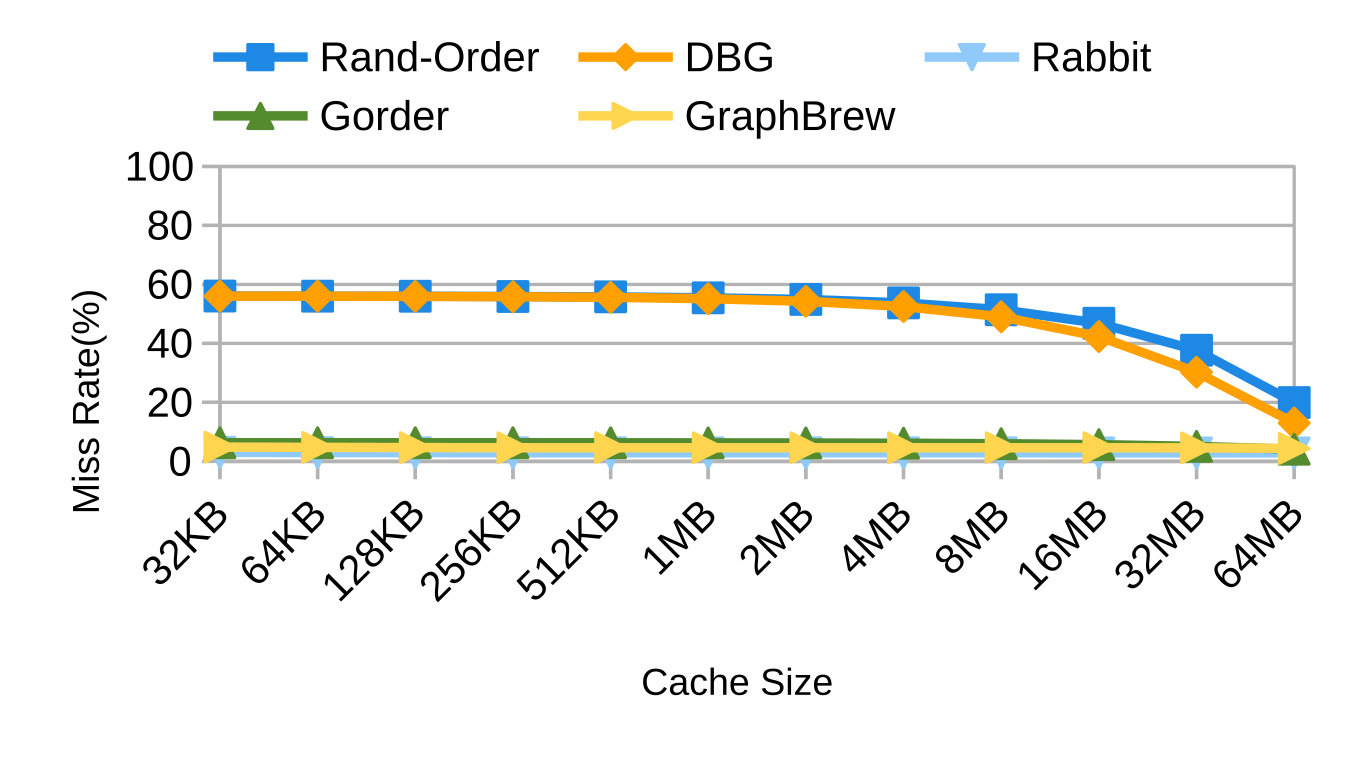
\includegraphics[width=\linewidth]{dataCharts/cache/road}
\label{fig:cache:road}
\end{subfigure}
\begin{subfigure}{.32\linewidth}
\caption{twitter}
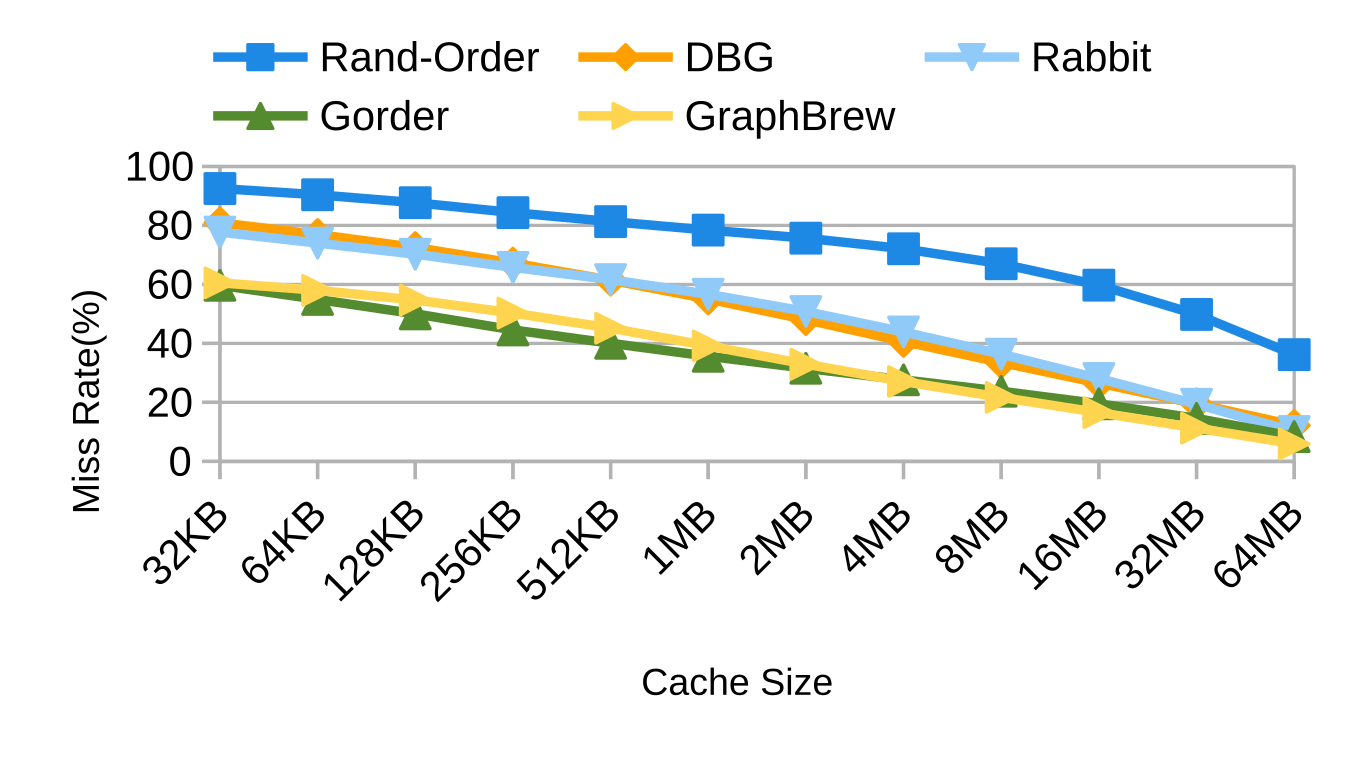
\includegraphics[width=\linewidth]{dataCharts/cache/twitter}
\label{fig:cache:twitter}
\end{subfigure}
\begin{subfigure}{.32\linewidth}
\caption{gplus}
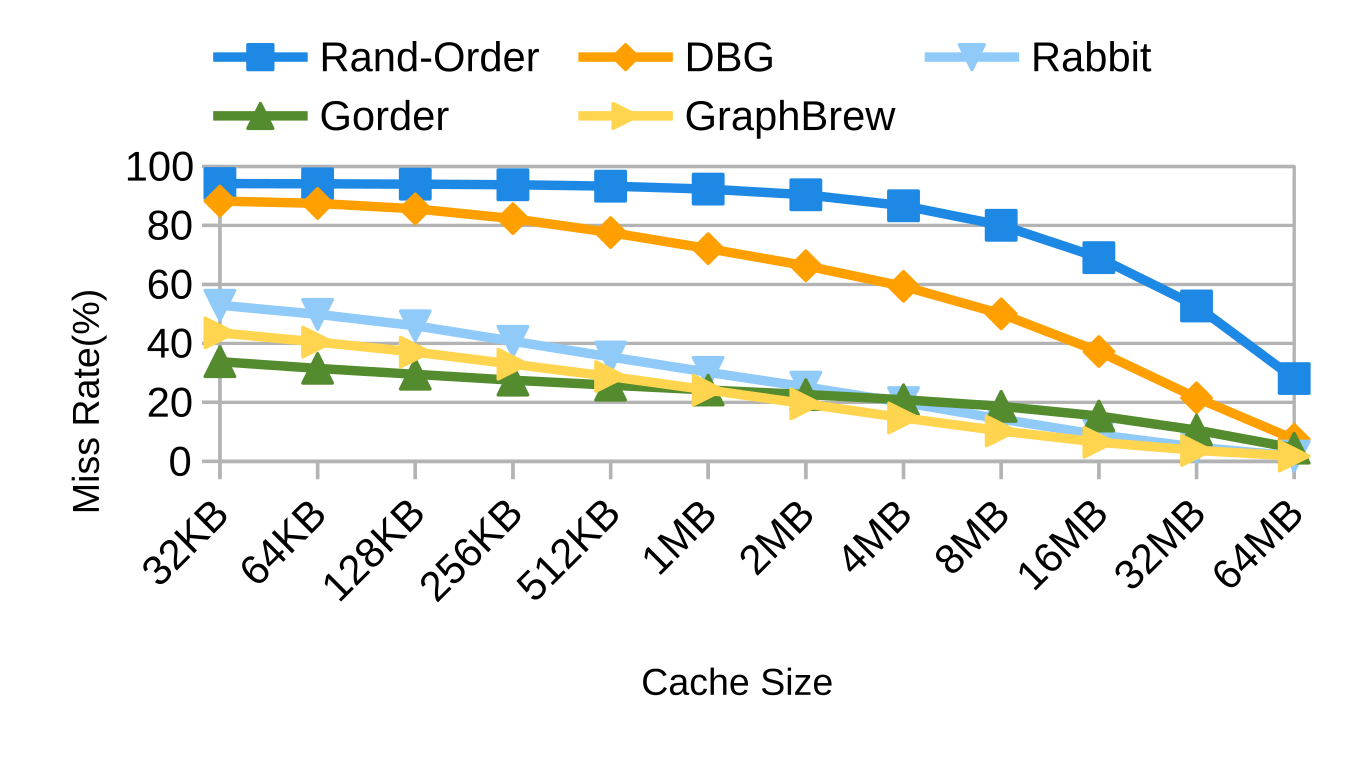
\includegraphics[width=\linewidth]{dataCharts/cache/gplus}
\label{fig:cache:gplus}
\end{subfigure}
%
\begin{subfigure}{.32\linewidth}
\caption{wikipedia-link-en}
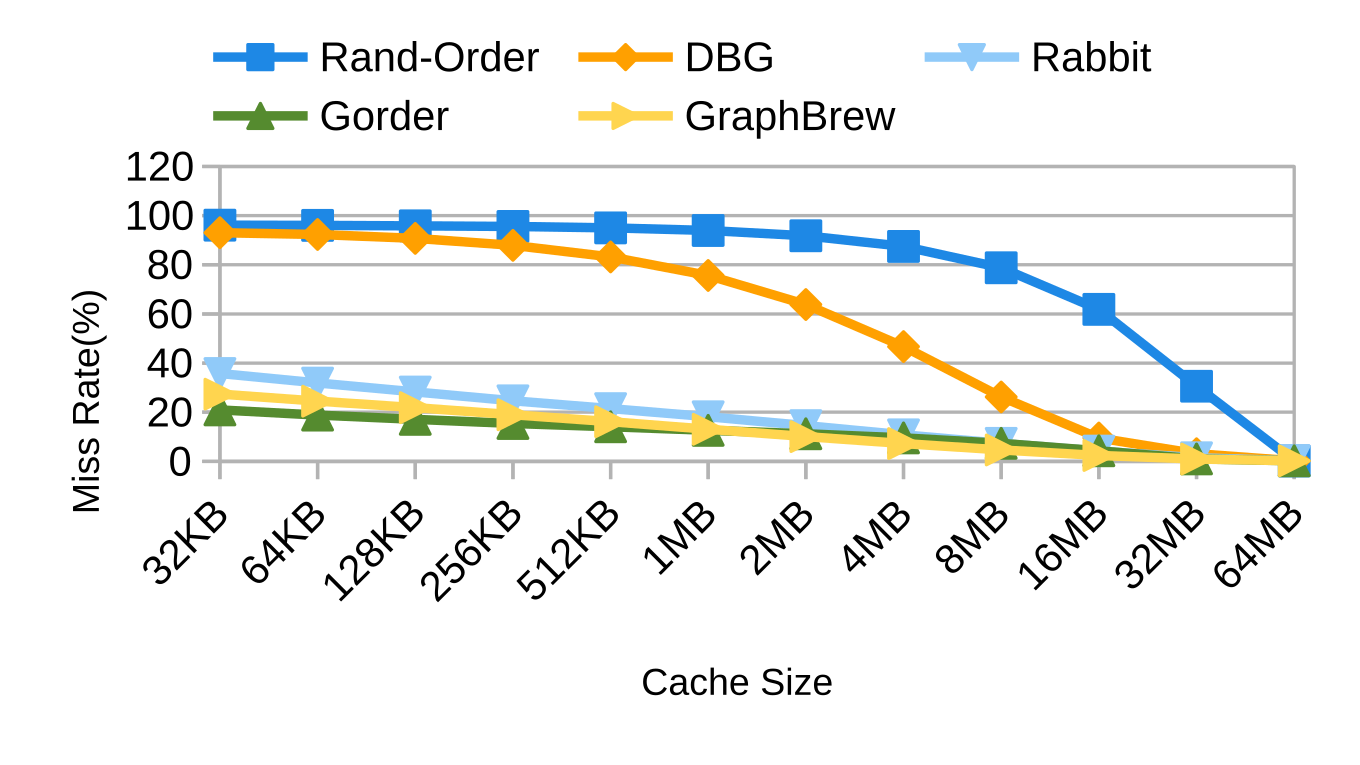
\includegraphics[width=\linewidth]{dataCharts/cache/wikipedia_link_en}
\label{fig:cache:wikipedia_link_en}
\end{subfigure}
\begin{subfigure}{.32\linewidth}
\caption{webbase-2001}
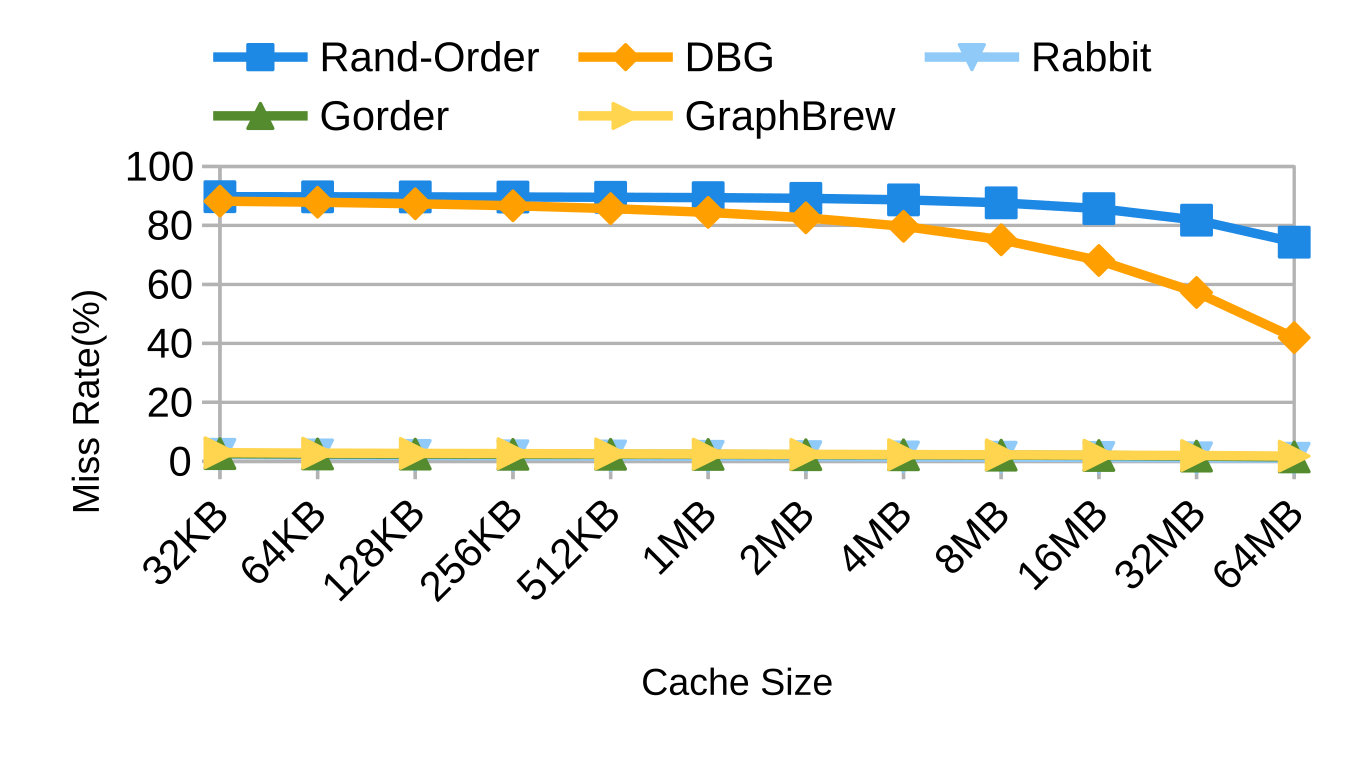
\includegraphics[width=\linewidth]{dataCharts/cache/Webbase-2001}
\label{fig:cache:Webbase-2001}
\end{subfigure}
\begin{subfigure}{.32\linewidth}
\caption{Geometric Mean (GM)}
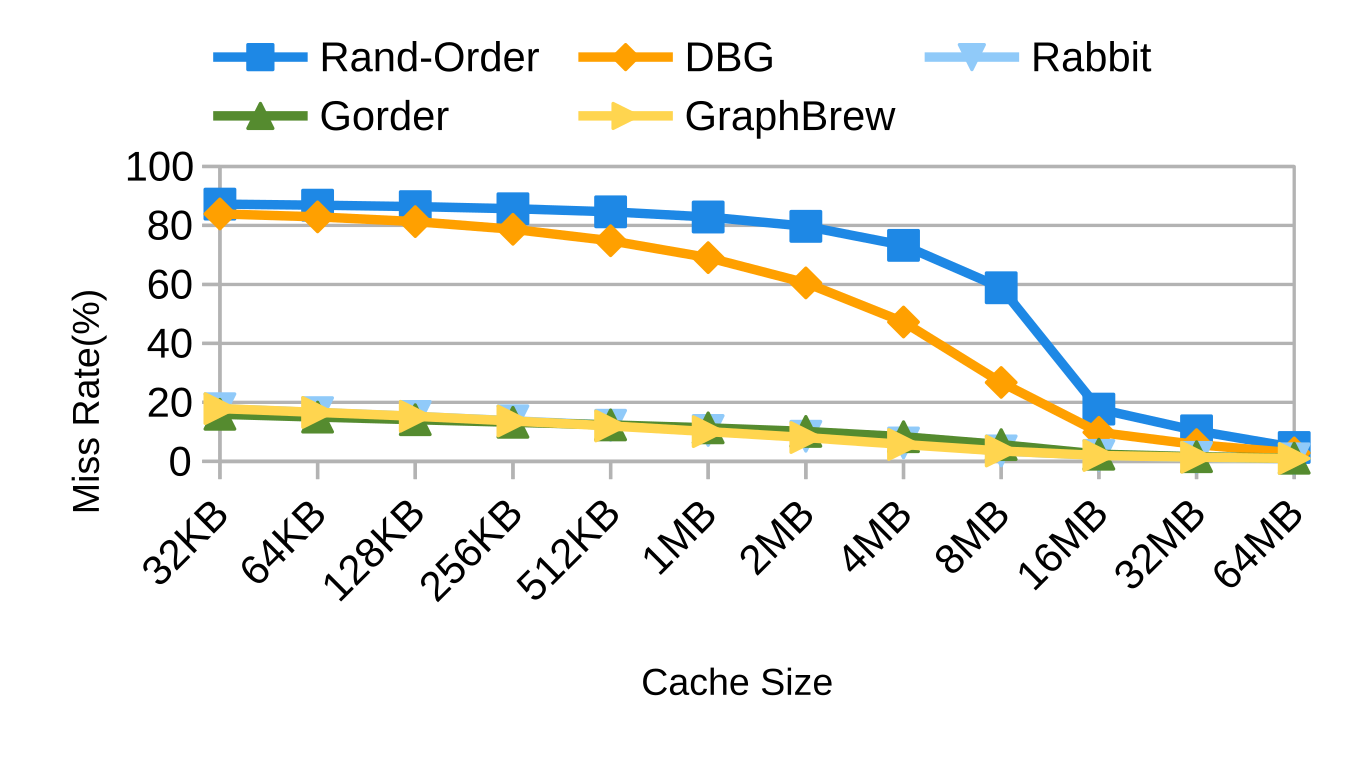
\includegraphics[width=\linewidth]{dataCharts/cache/cacheGM}
\label{fig:cache:cacheGM}
\end{subfigure}

\caption{Cache performance, and miss rate. Results of simulating PageRank (PR) pull approach on a simple trace driven cache simulator.}
\label{fig:cache:performance}
\end{figure*}

\begin{figure*}[ht]
\centering
\begin{subfigure}{.32\linewidth}
\caption{Breadth First Search (BFS)}
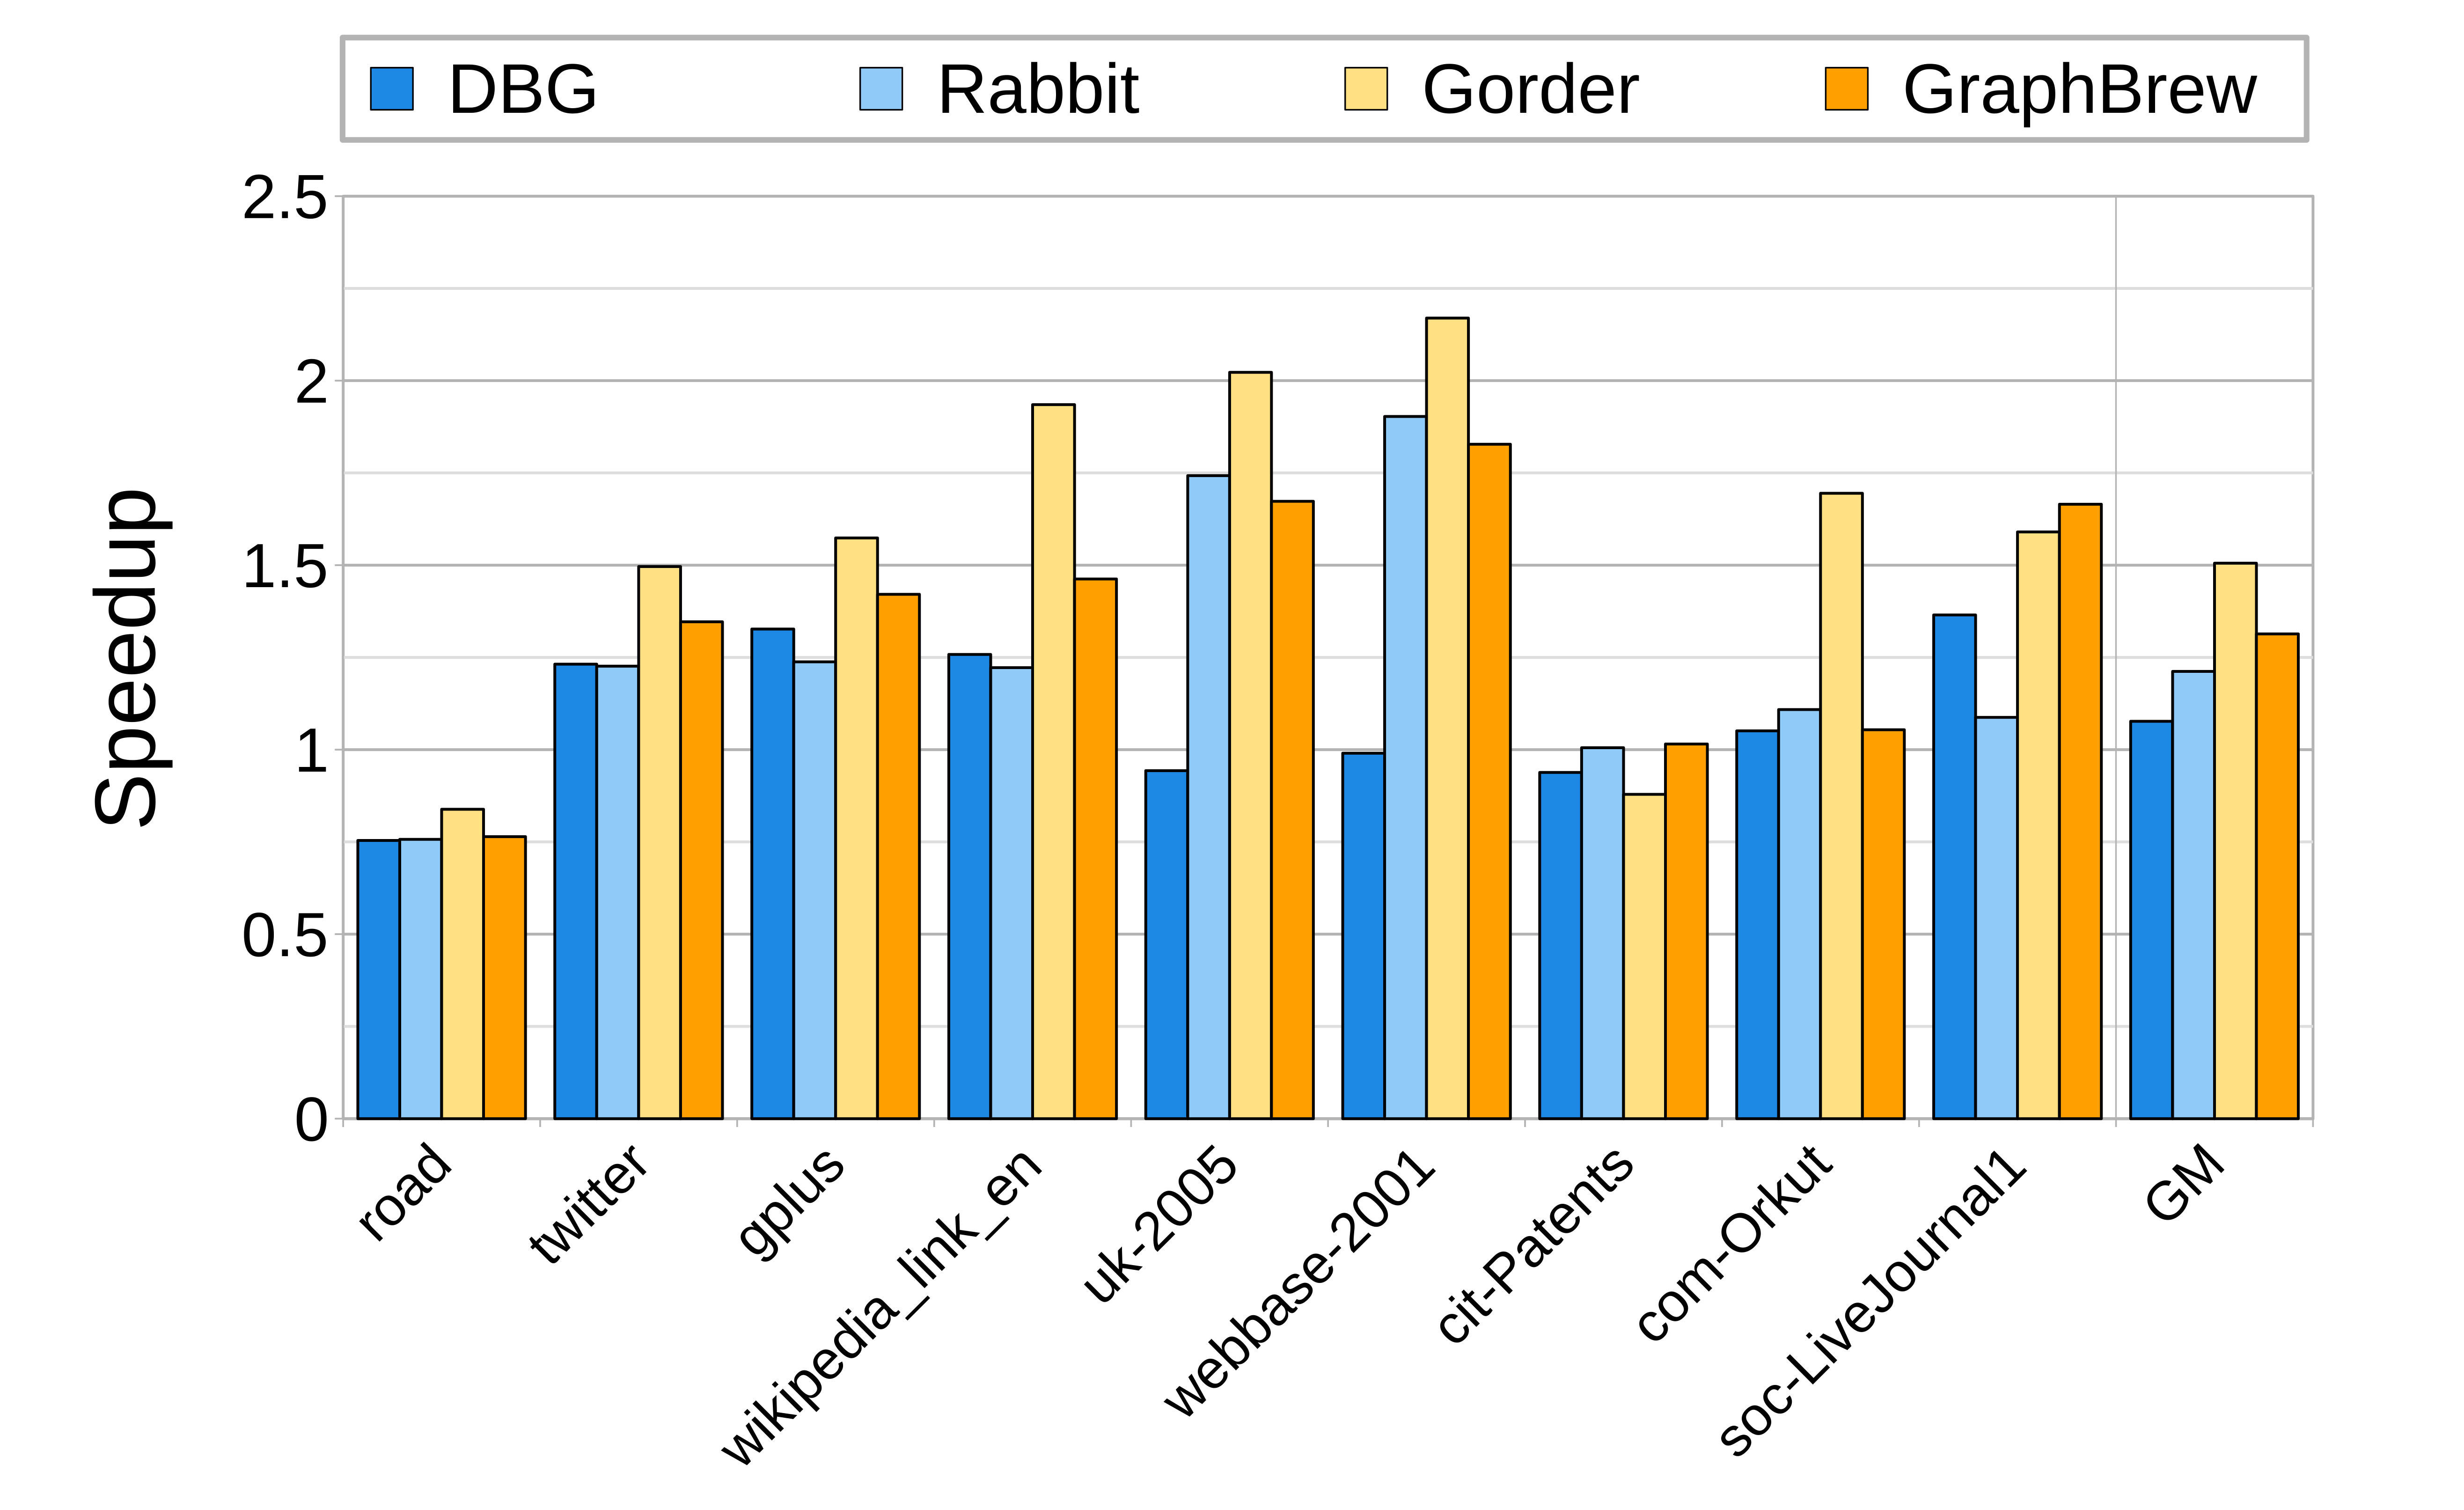
\includegraphics[width=\linewidth]{dataCharts/speedup/BFS}
\label{fig:speedups:BFS}
\end{subfigure}
\begin{subfigure}{.32\linewidth}
\caption{PageRank (PR)}
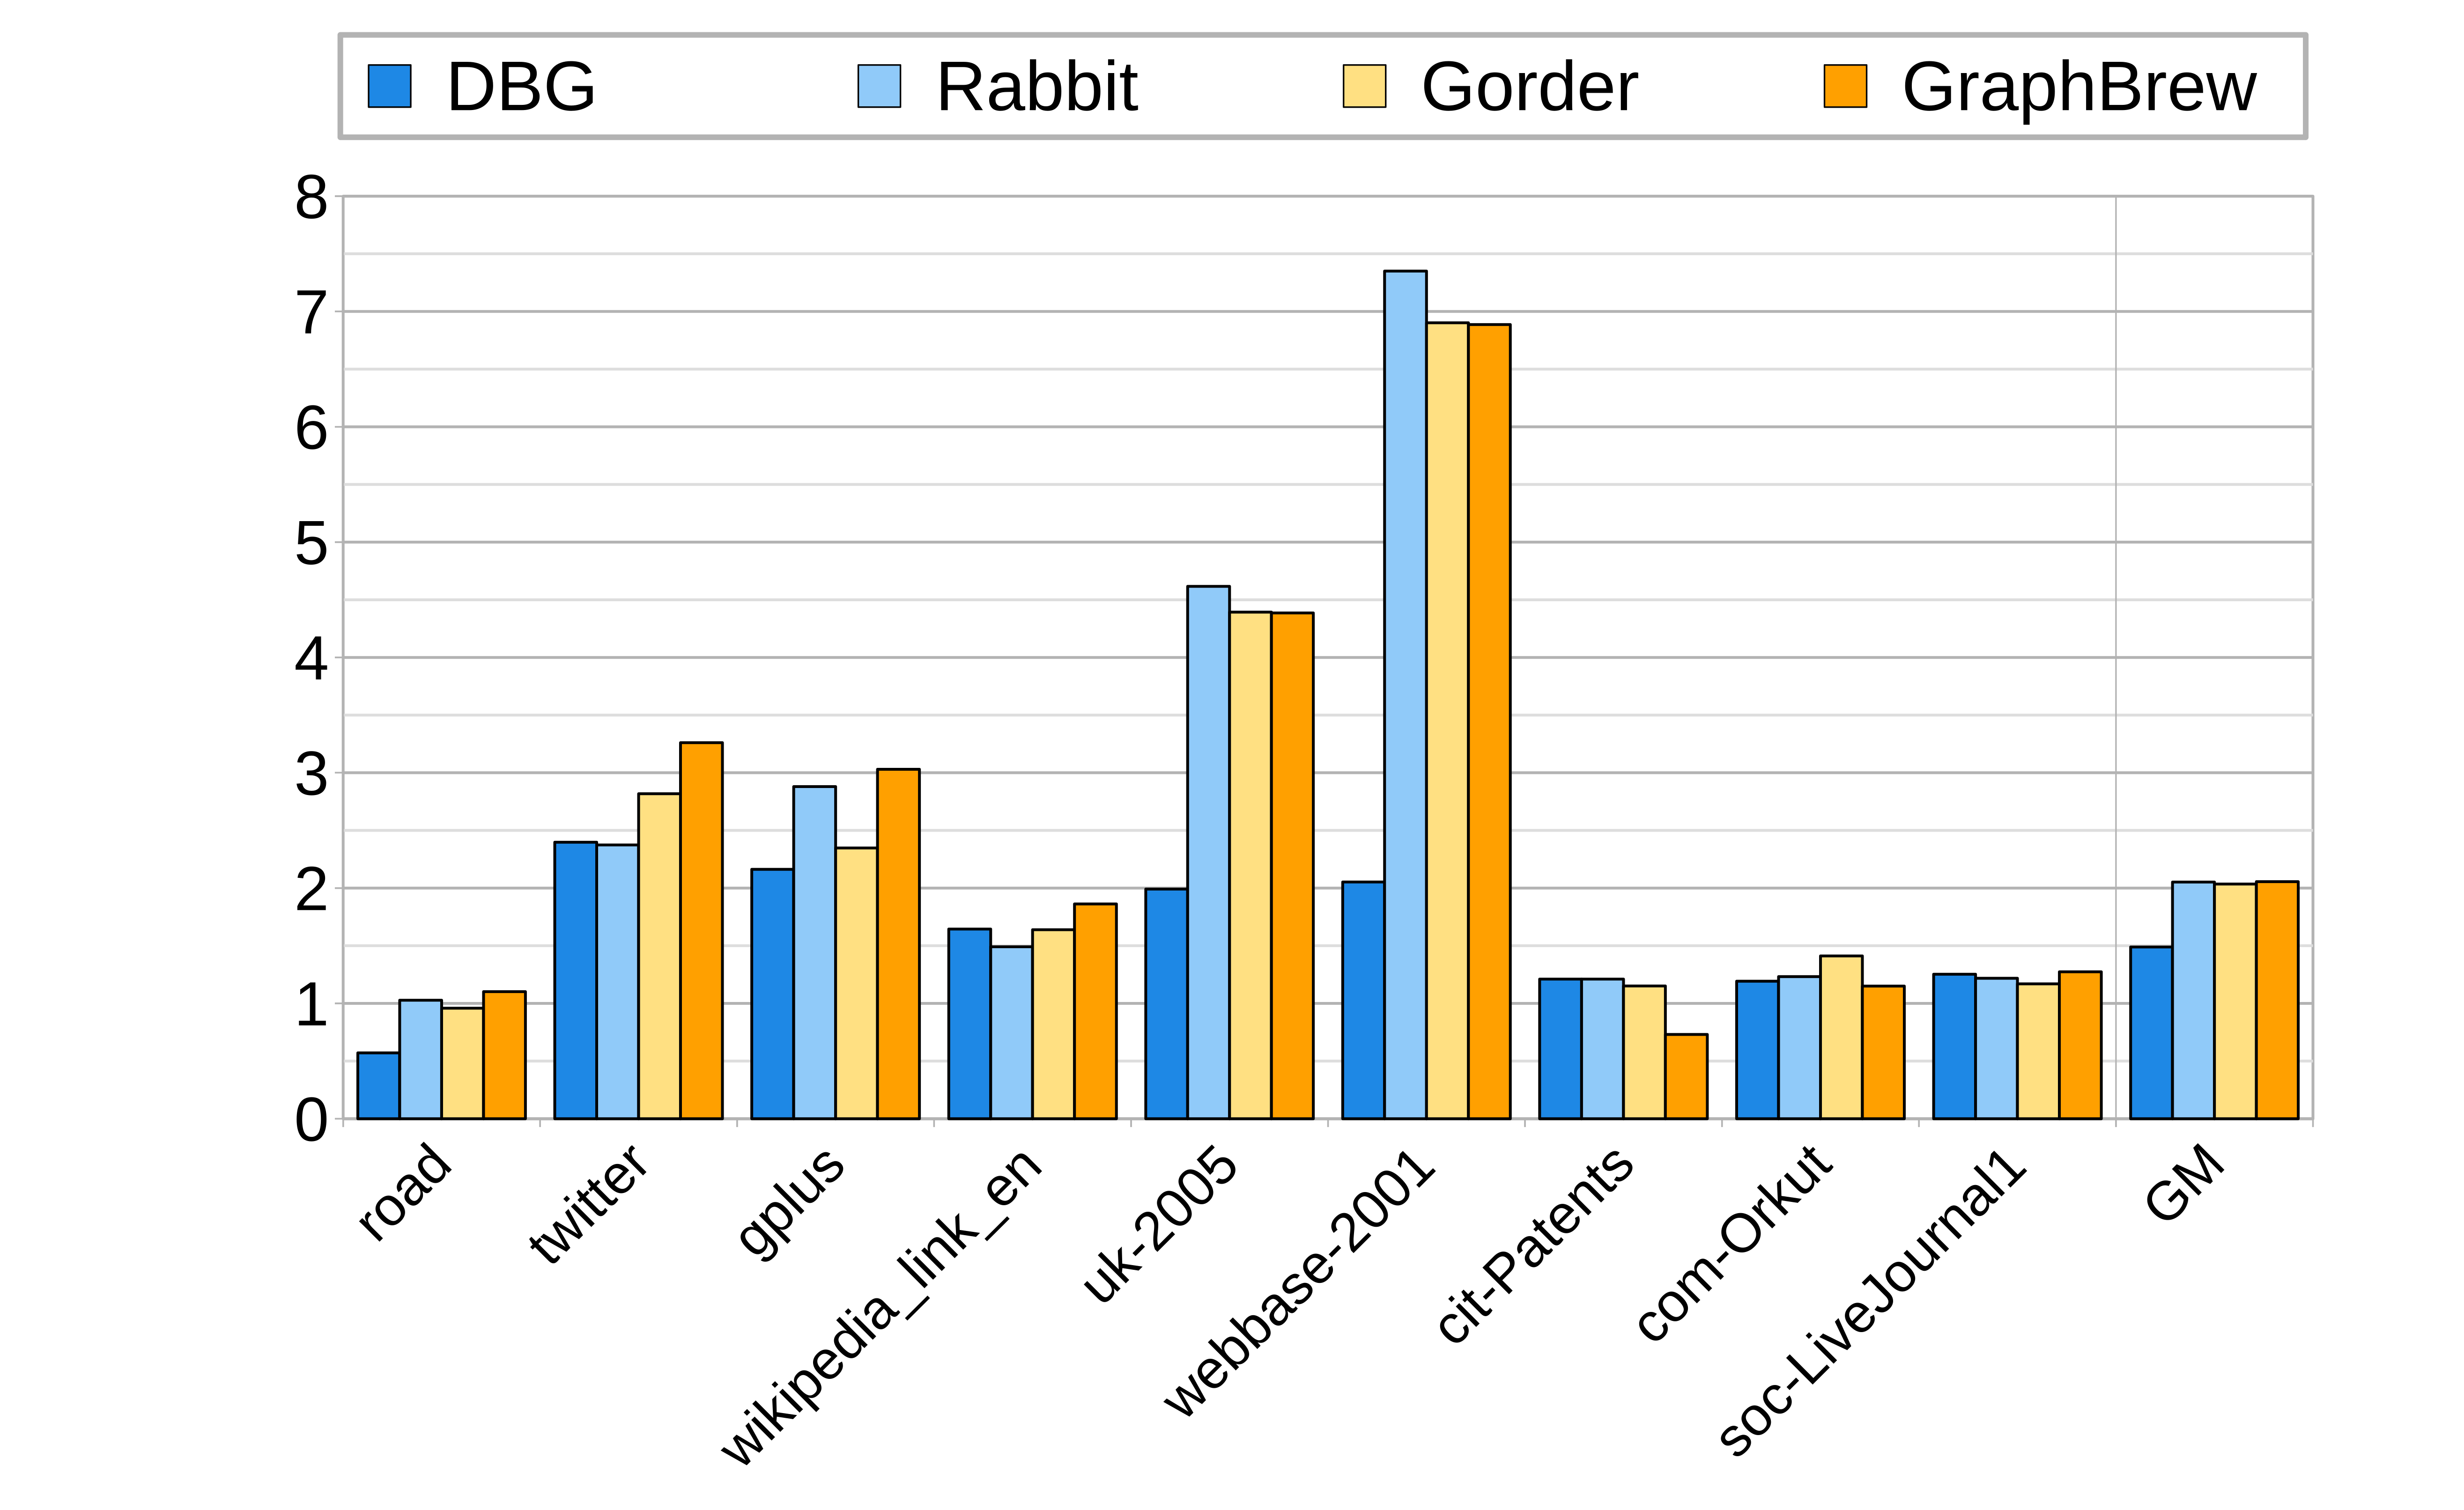
\includegraphics[width=\linewidth]{dataCharts/speedup/PR}
\label{fig:speedups:PR}
\end{subfigure}
\begin{subfigure}{.32\linewidth}
\caption{Single Source Shortest Path (SSSP)}
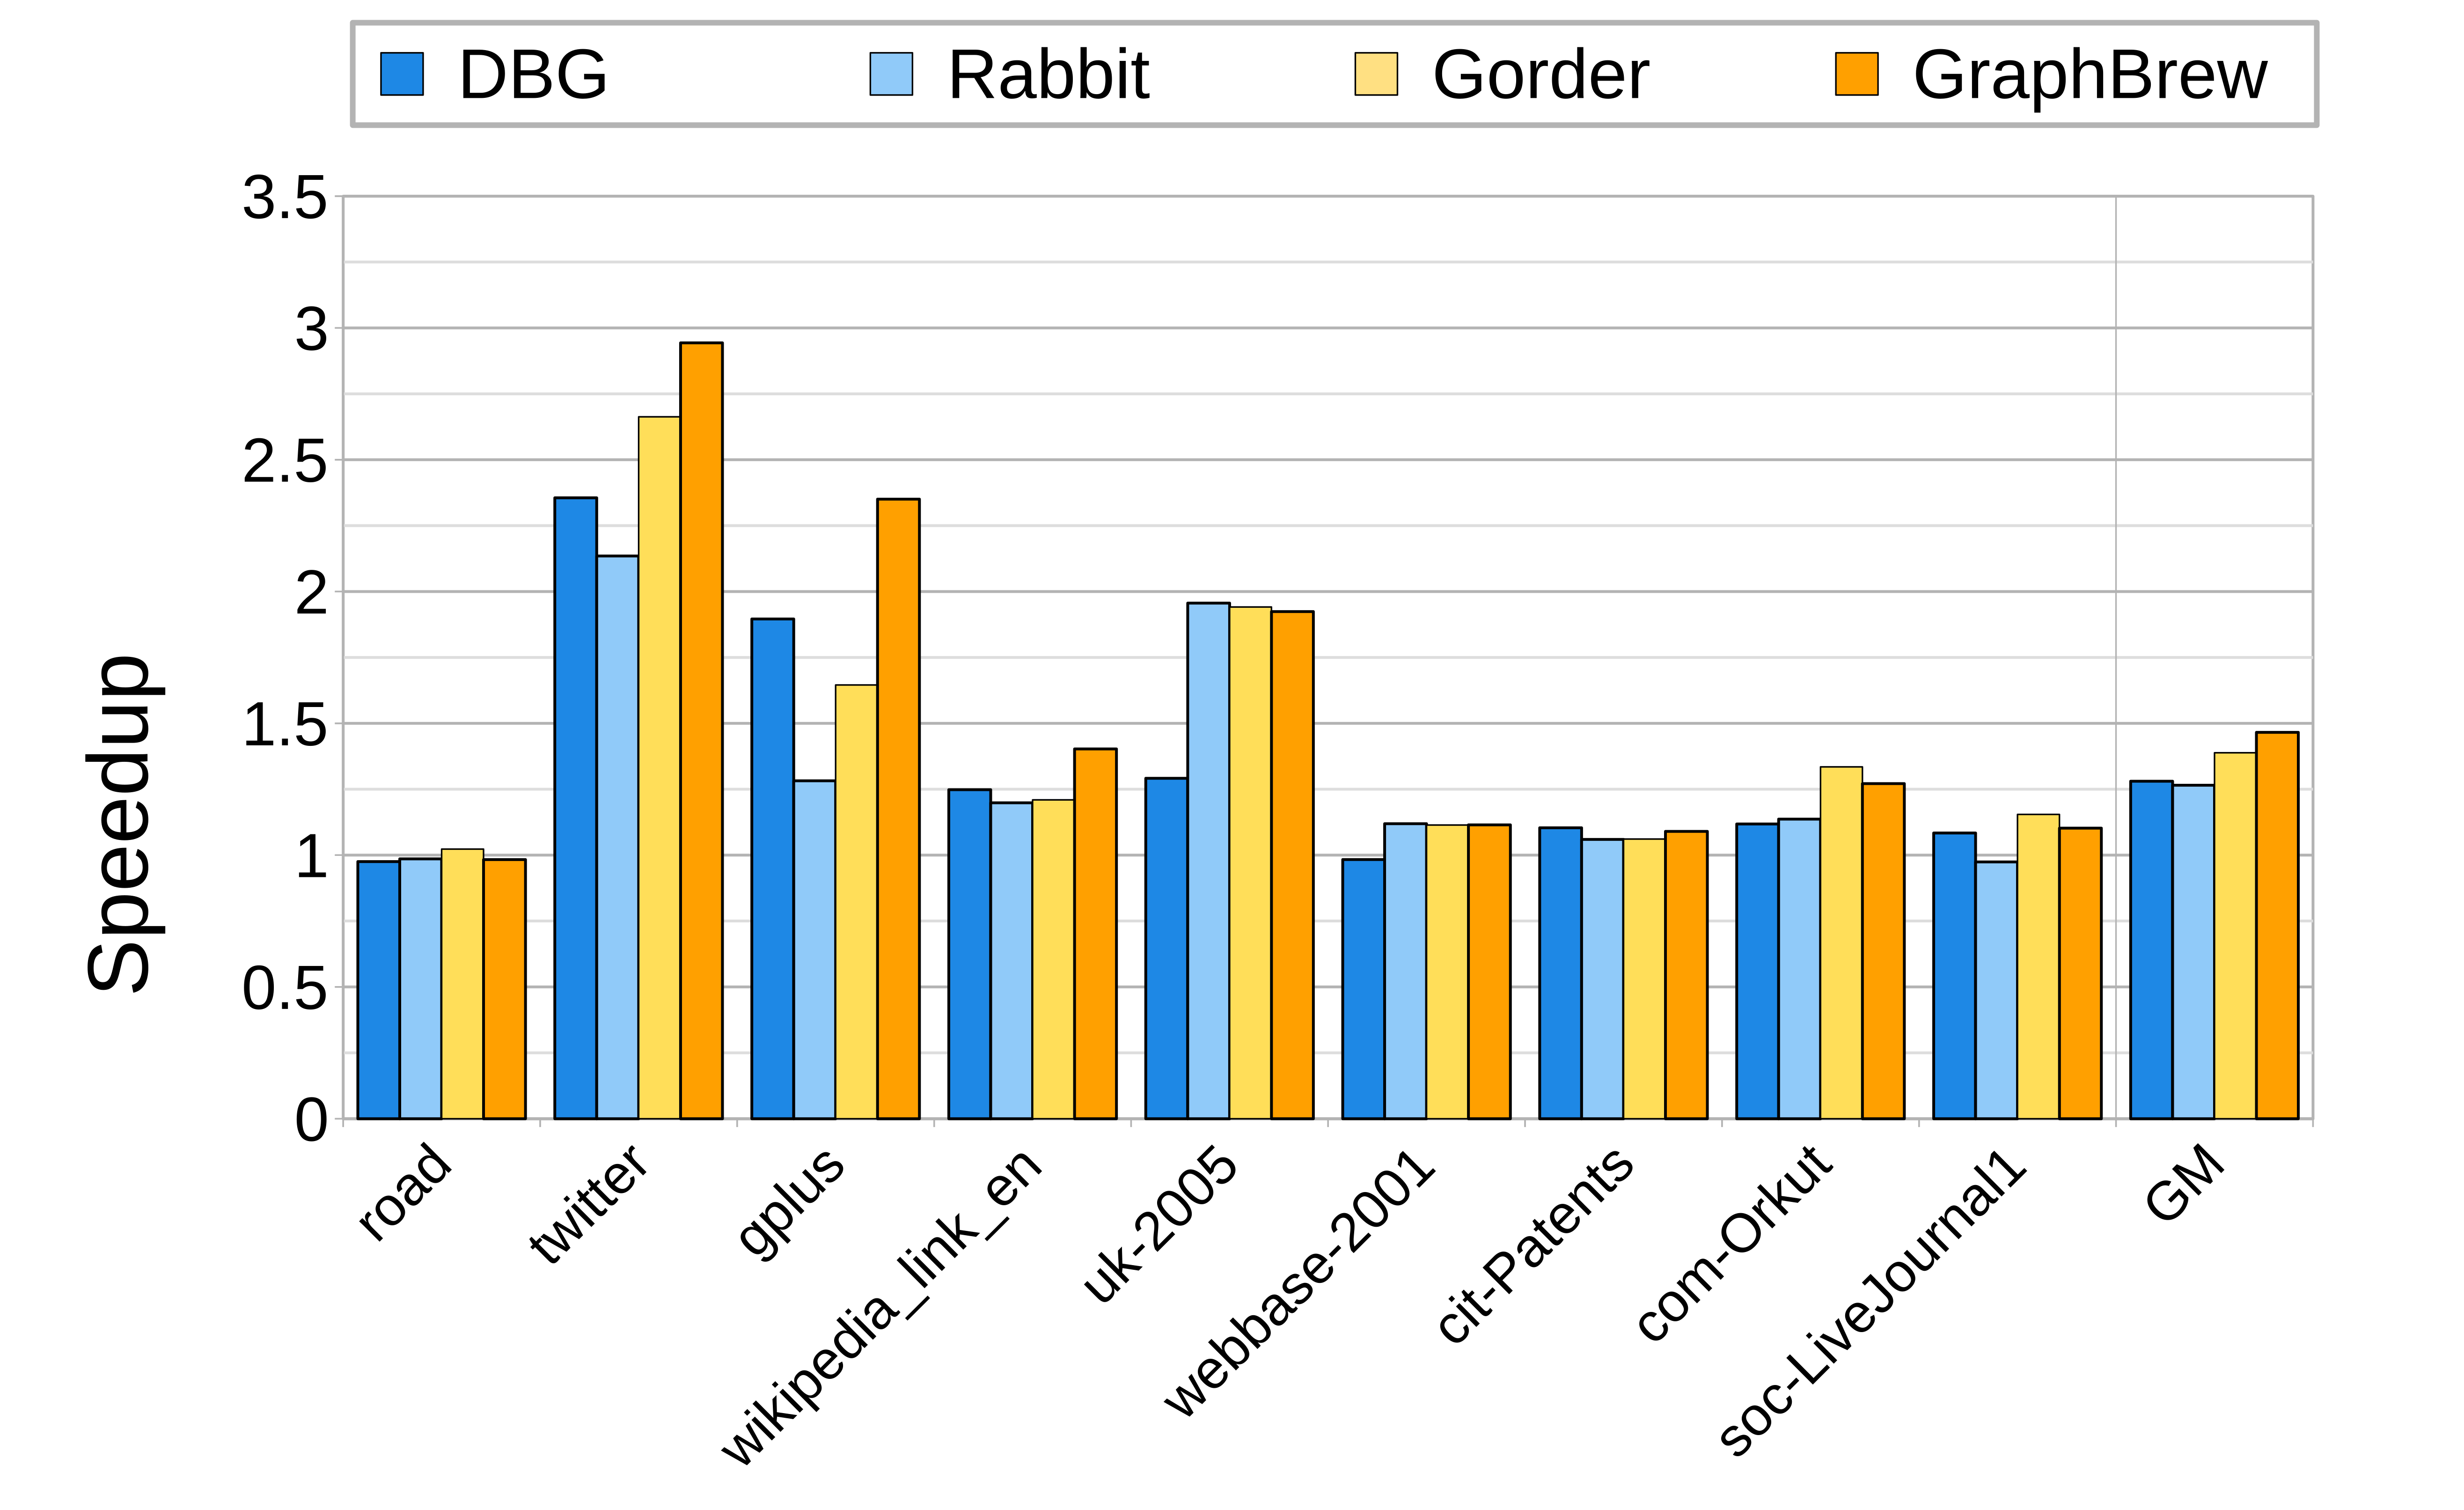
\includegraphics[width=\linewidth]{dataCharts/speedup/SSSP}
\label{fig:speedups:SSSP}
\end{subfigure}

\begin{subfigure}{.32\linewidth}
\caption{Sparse Matrix-Vector Multiplication (SpMV)}

\includegraphics[width=\linewidth]{dataCharts/speedup/SPMV}
\label{fig:speedups:SPMV}
\end{subfigure}
\begin{subfigure}{.32\linewidth}
\caption{Connected Components (CC)}
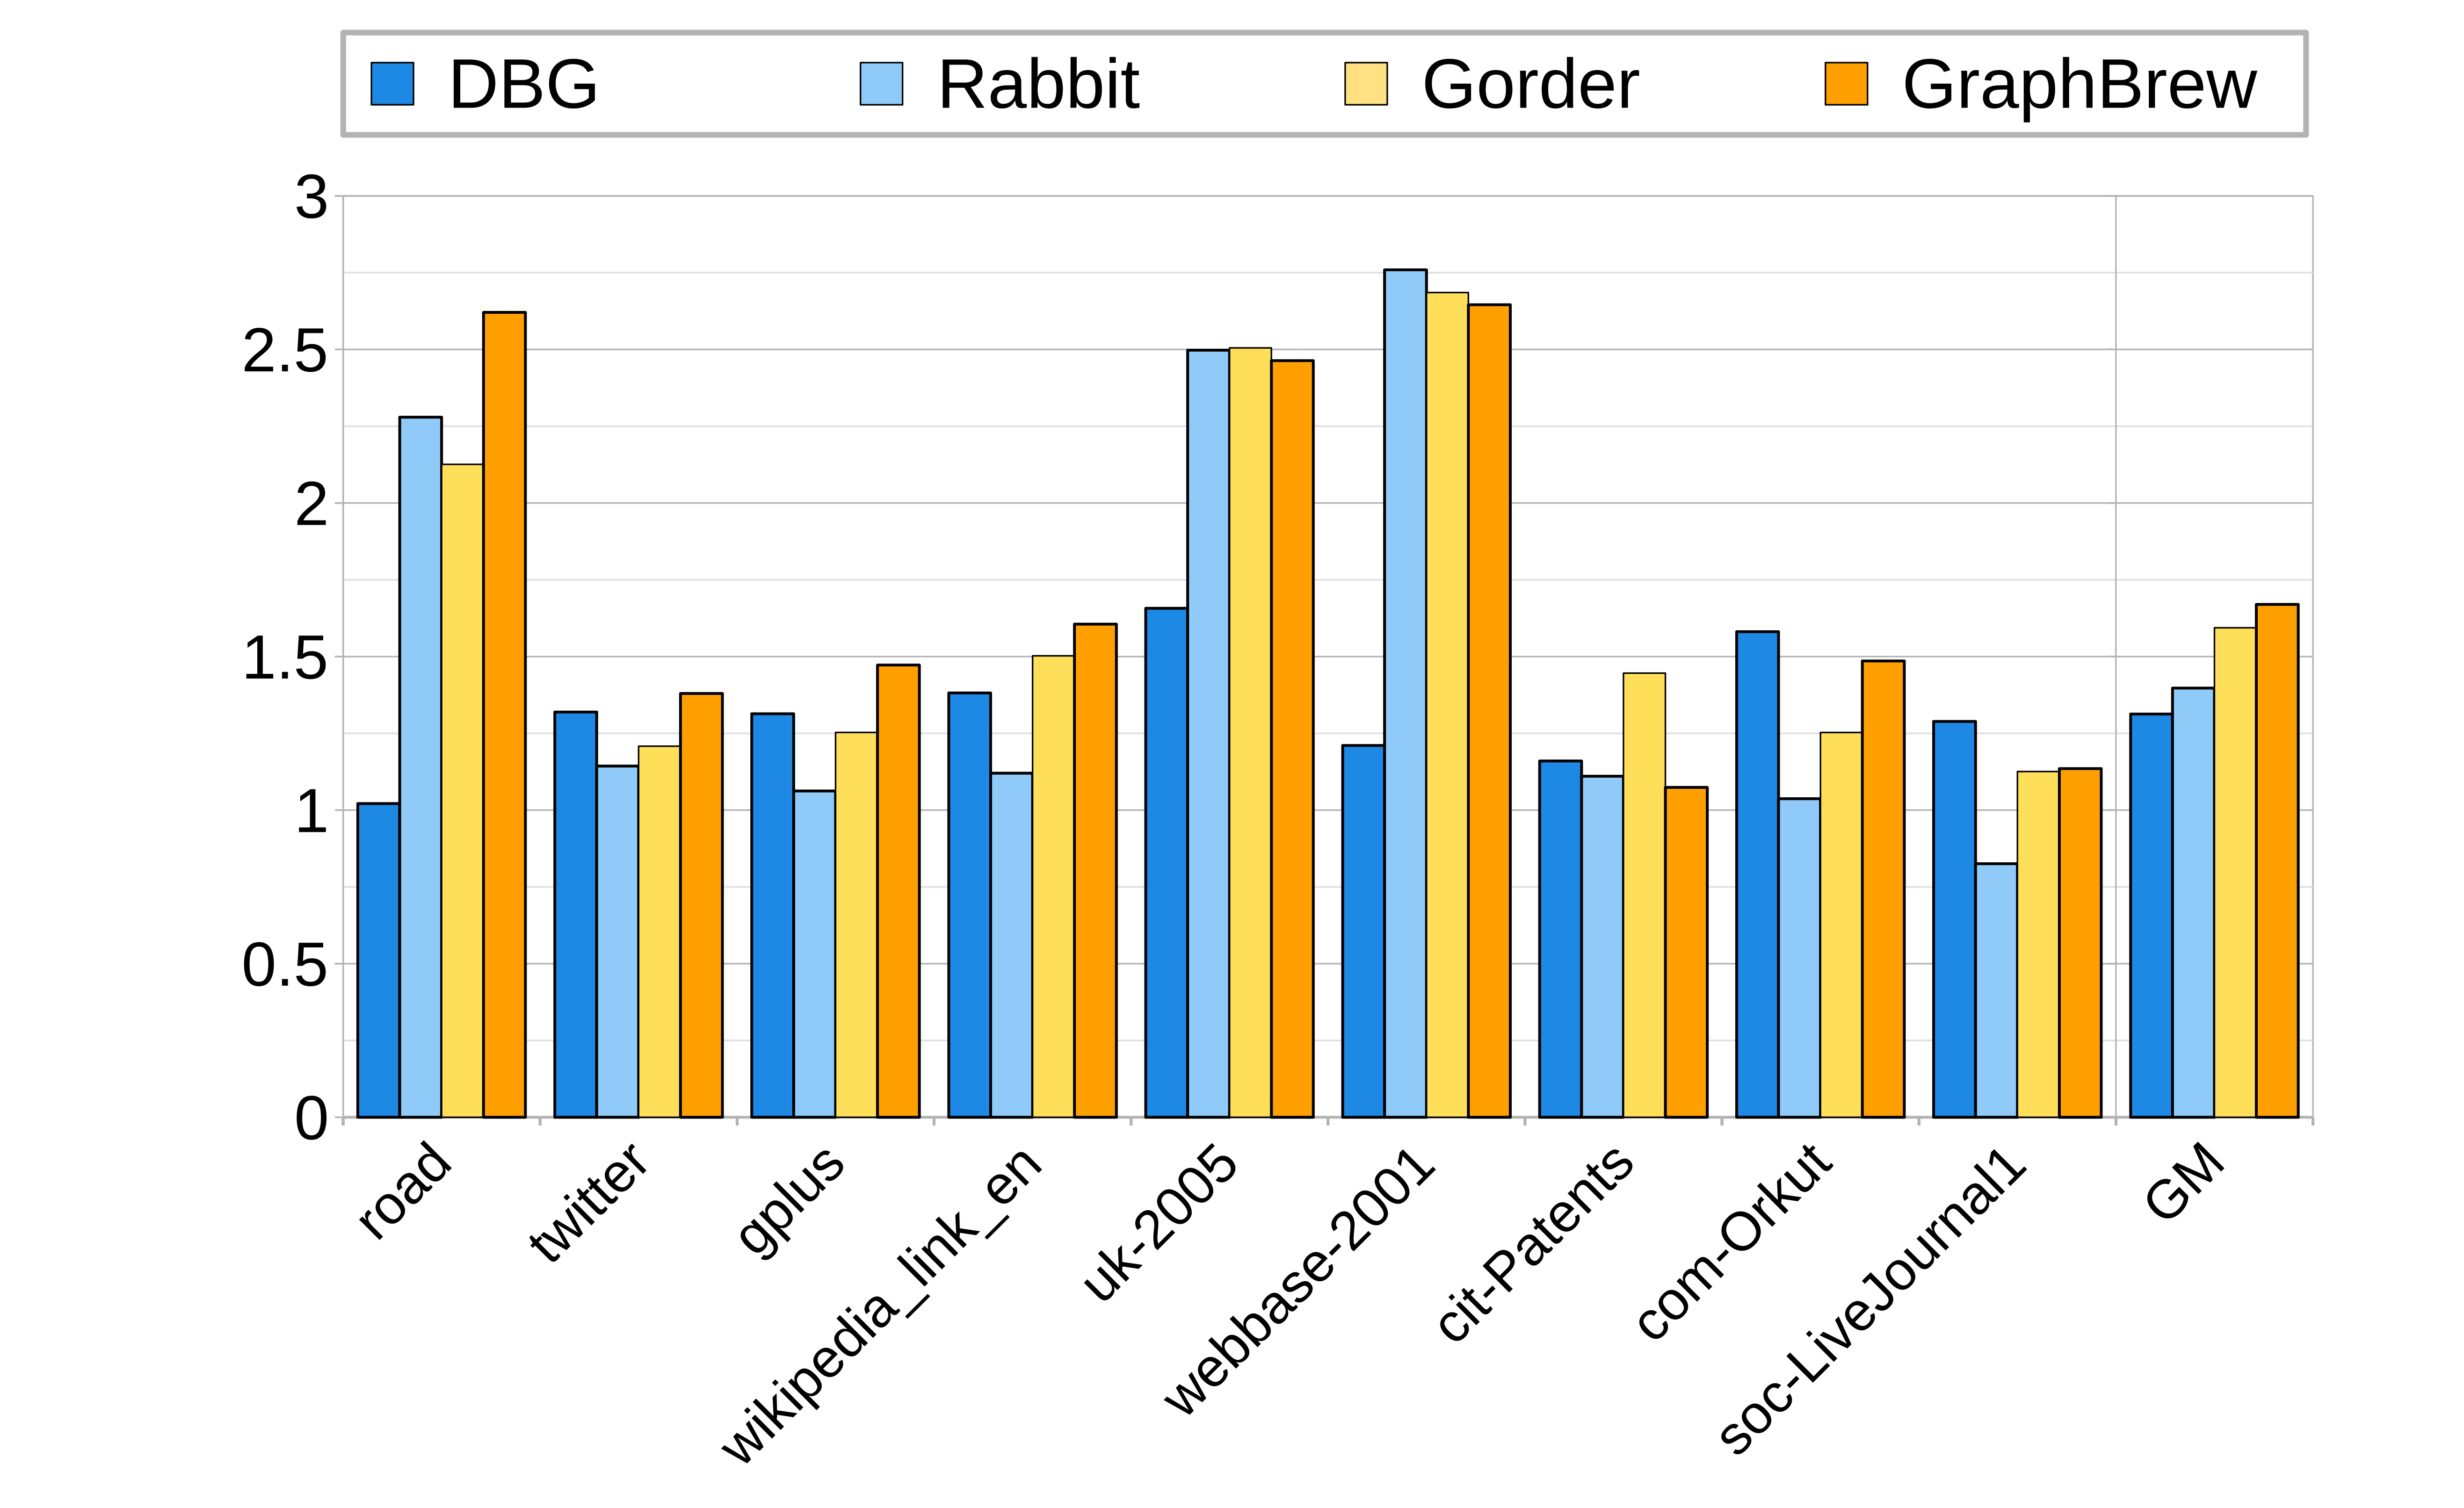
\includegraphics[width=\linewidth]{dataCharts/speedup/CC}
\label{fig:speedups:CC}
\end{subfigure}
\begin{subfigure}{.32\linewidth}
\caption{Aggregated speedup for graph data-sets }
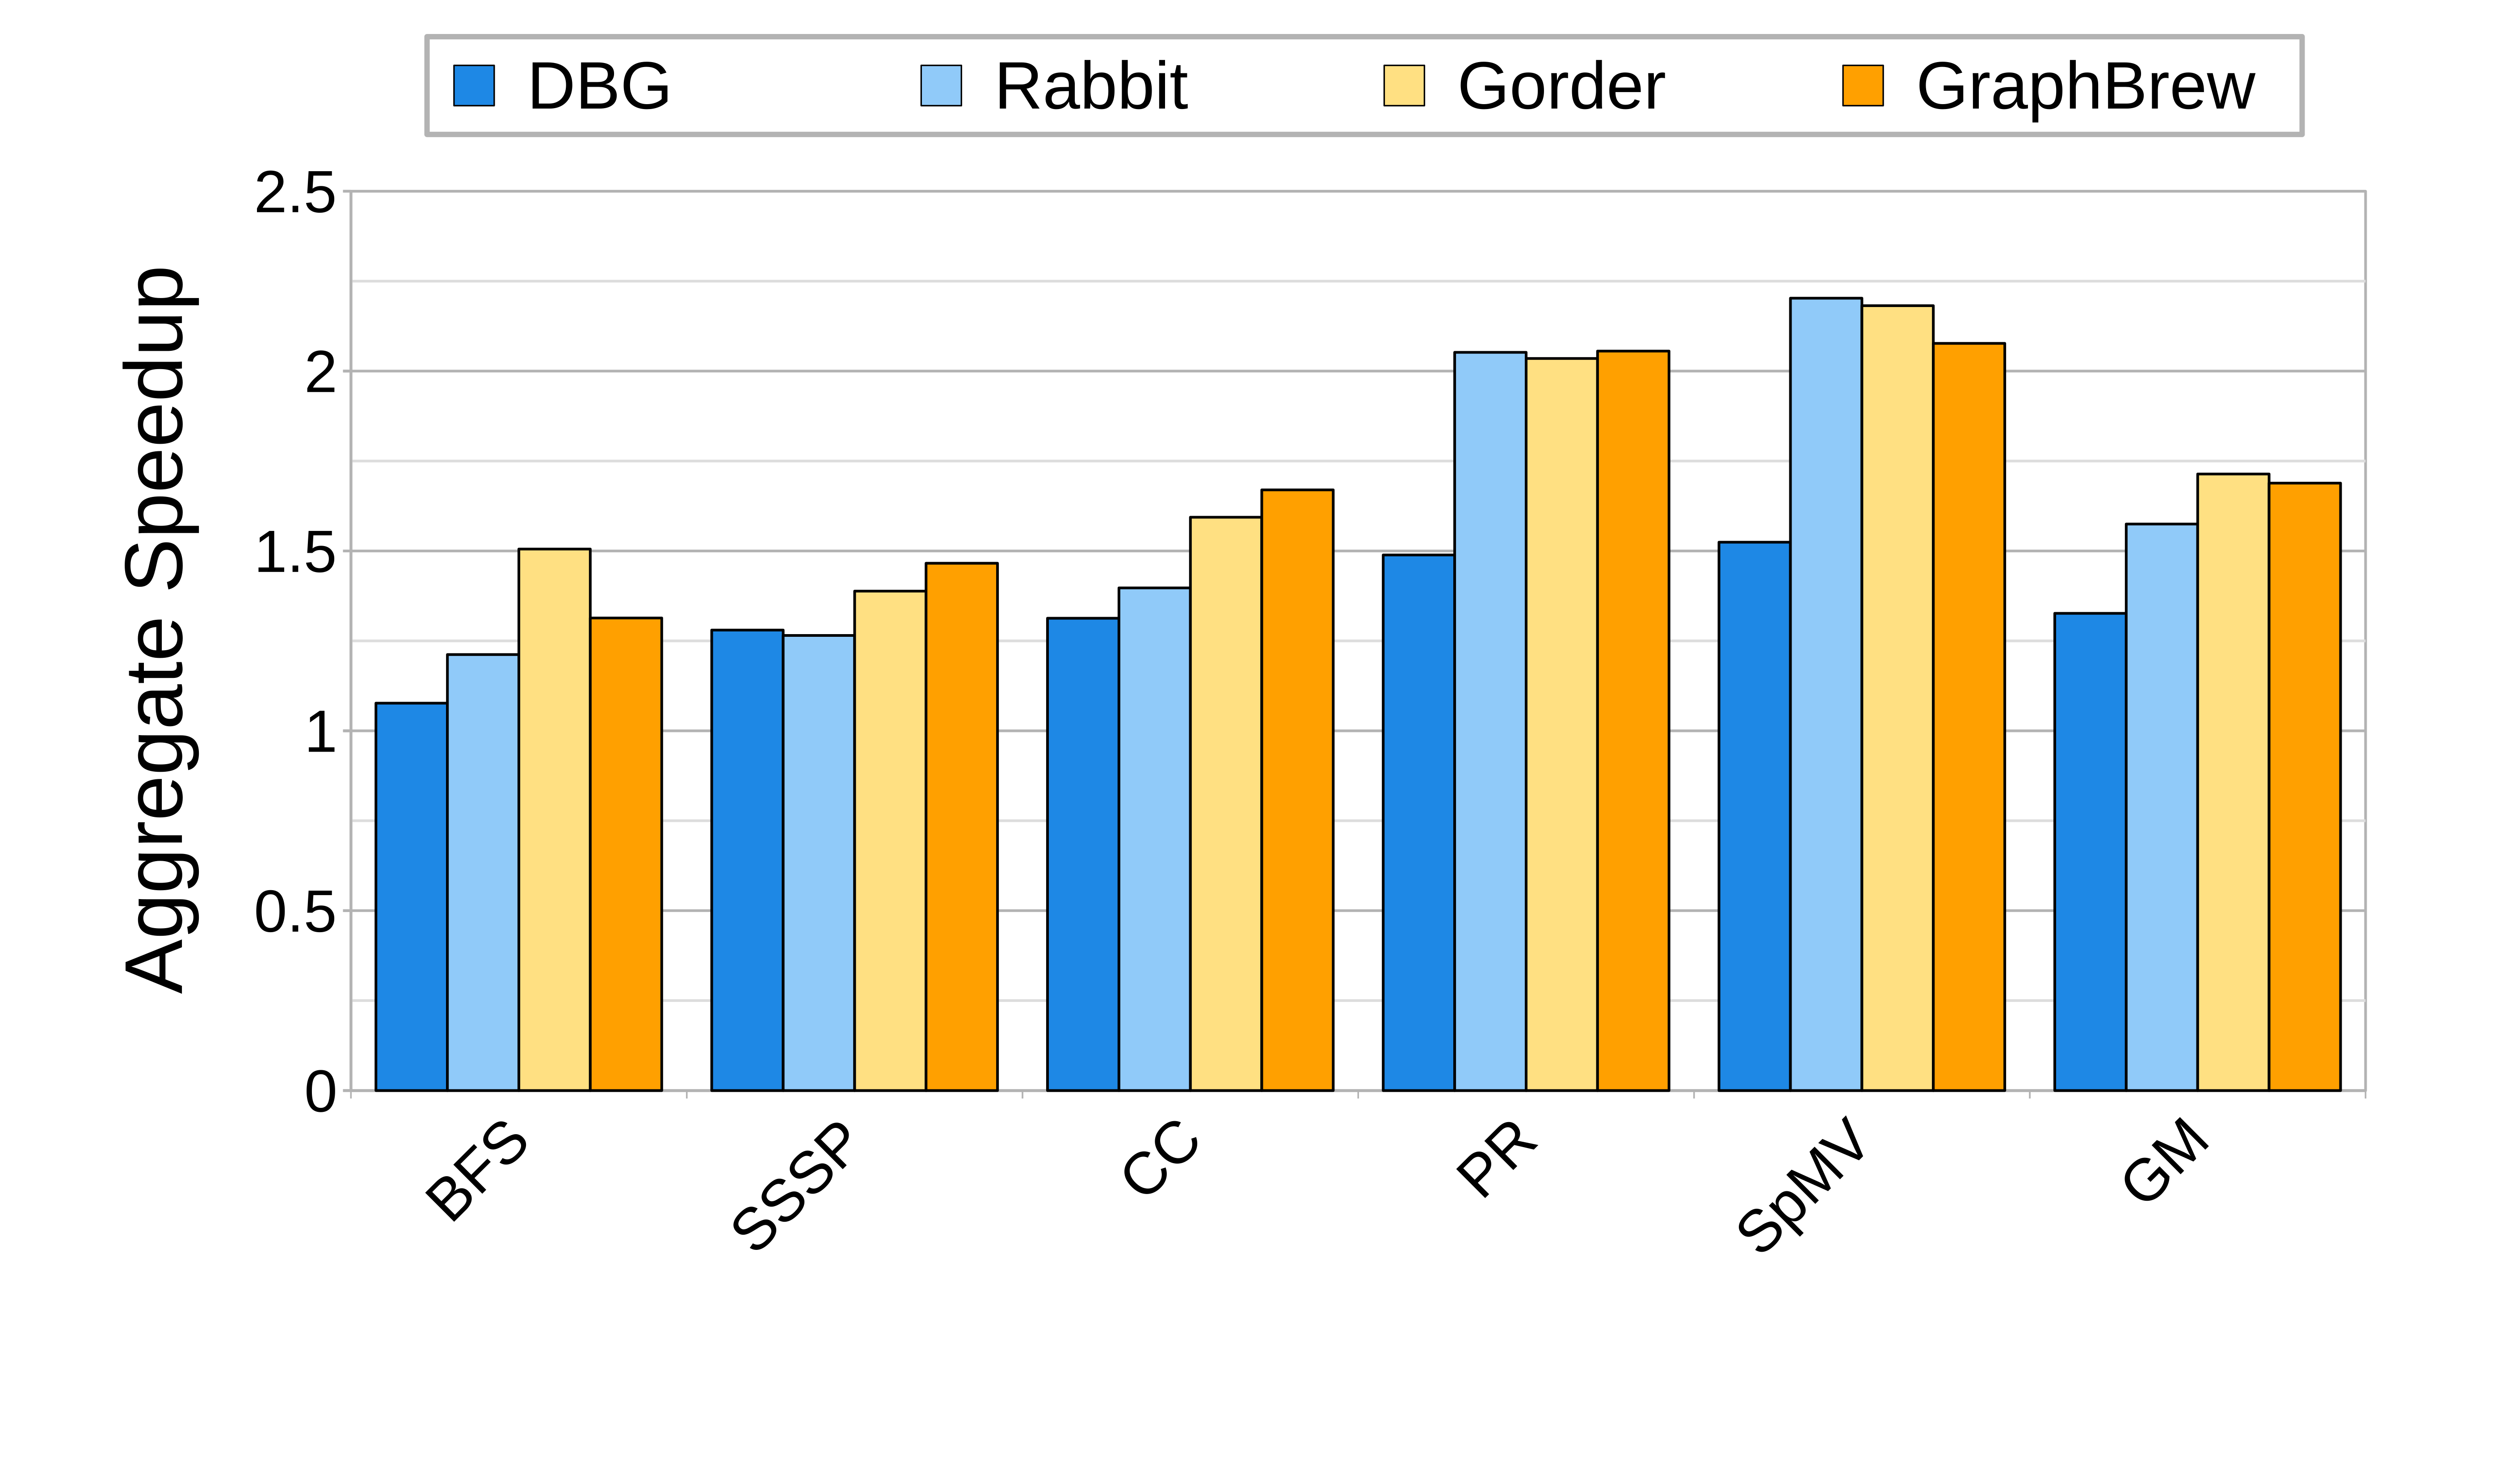
\includegraphics[width=\linewidth]{dataCharts/speedup/aggregateSpeedups}
\label{fig:aggregateSpeedups}
\end{subfigure}
\caption{Speedup comparison of GraphBrew lightweight reordering against other techniques: Data are normalized to run-time with the original graph random labeling performance.}
\label{fig:speedups}
\end{figure*}

\begin{figure*}[ht]
\centering
\begin{subfigure}{.32\linewidth}
\caption{Breadth First Search (BFS)}

\includegraphics[width=\linewidth]{dataCharts/trials/BFS}
\label{fig:trials:BFS}
\end{subfigure}
\begin{subfigure}{.32\linewidth}
\caption{PageRank (PR)}

\includegraphics[width=\linewidth]{dataCharts/trials/PR}
\label{fig:trials:PR}
\end{subfigure}
\begin{subfigure}{.32\linewidth}
\caption{Single Source Shortest Path (SSSP)}

\includegraphics[width=\linewidth]{dataCharts/trials/SSSP}
\label{fig:trials:SSSP}
\end{subfigure}

\begin{subfigure}{.32\linewidth}
\caption{Sparse Matrix-Vector Multiplication (SpMV)}
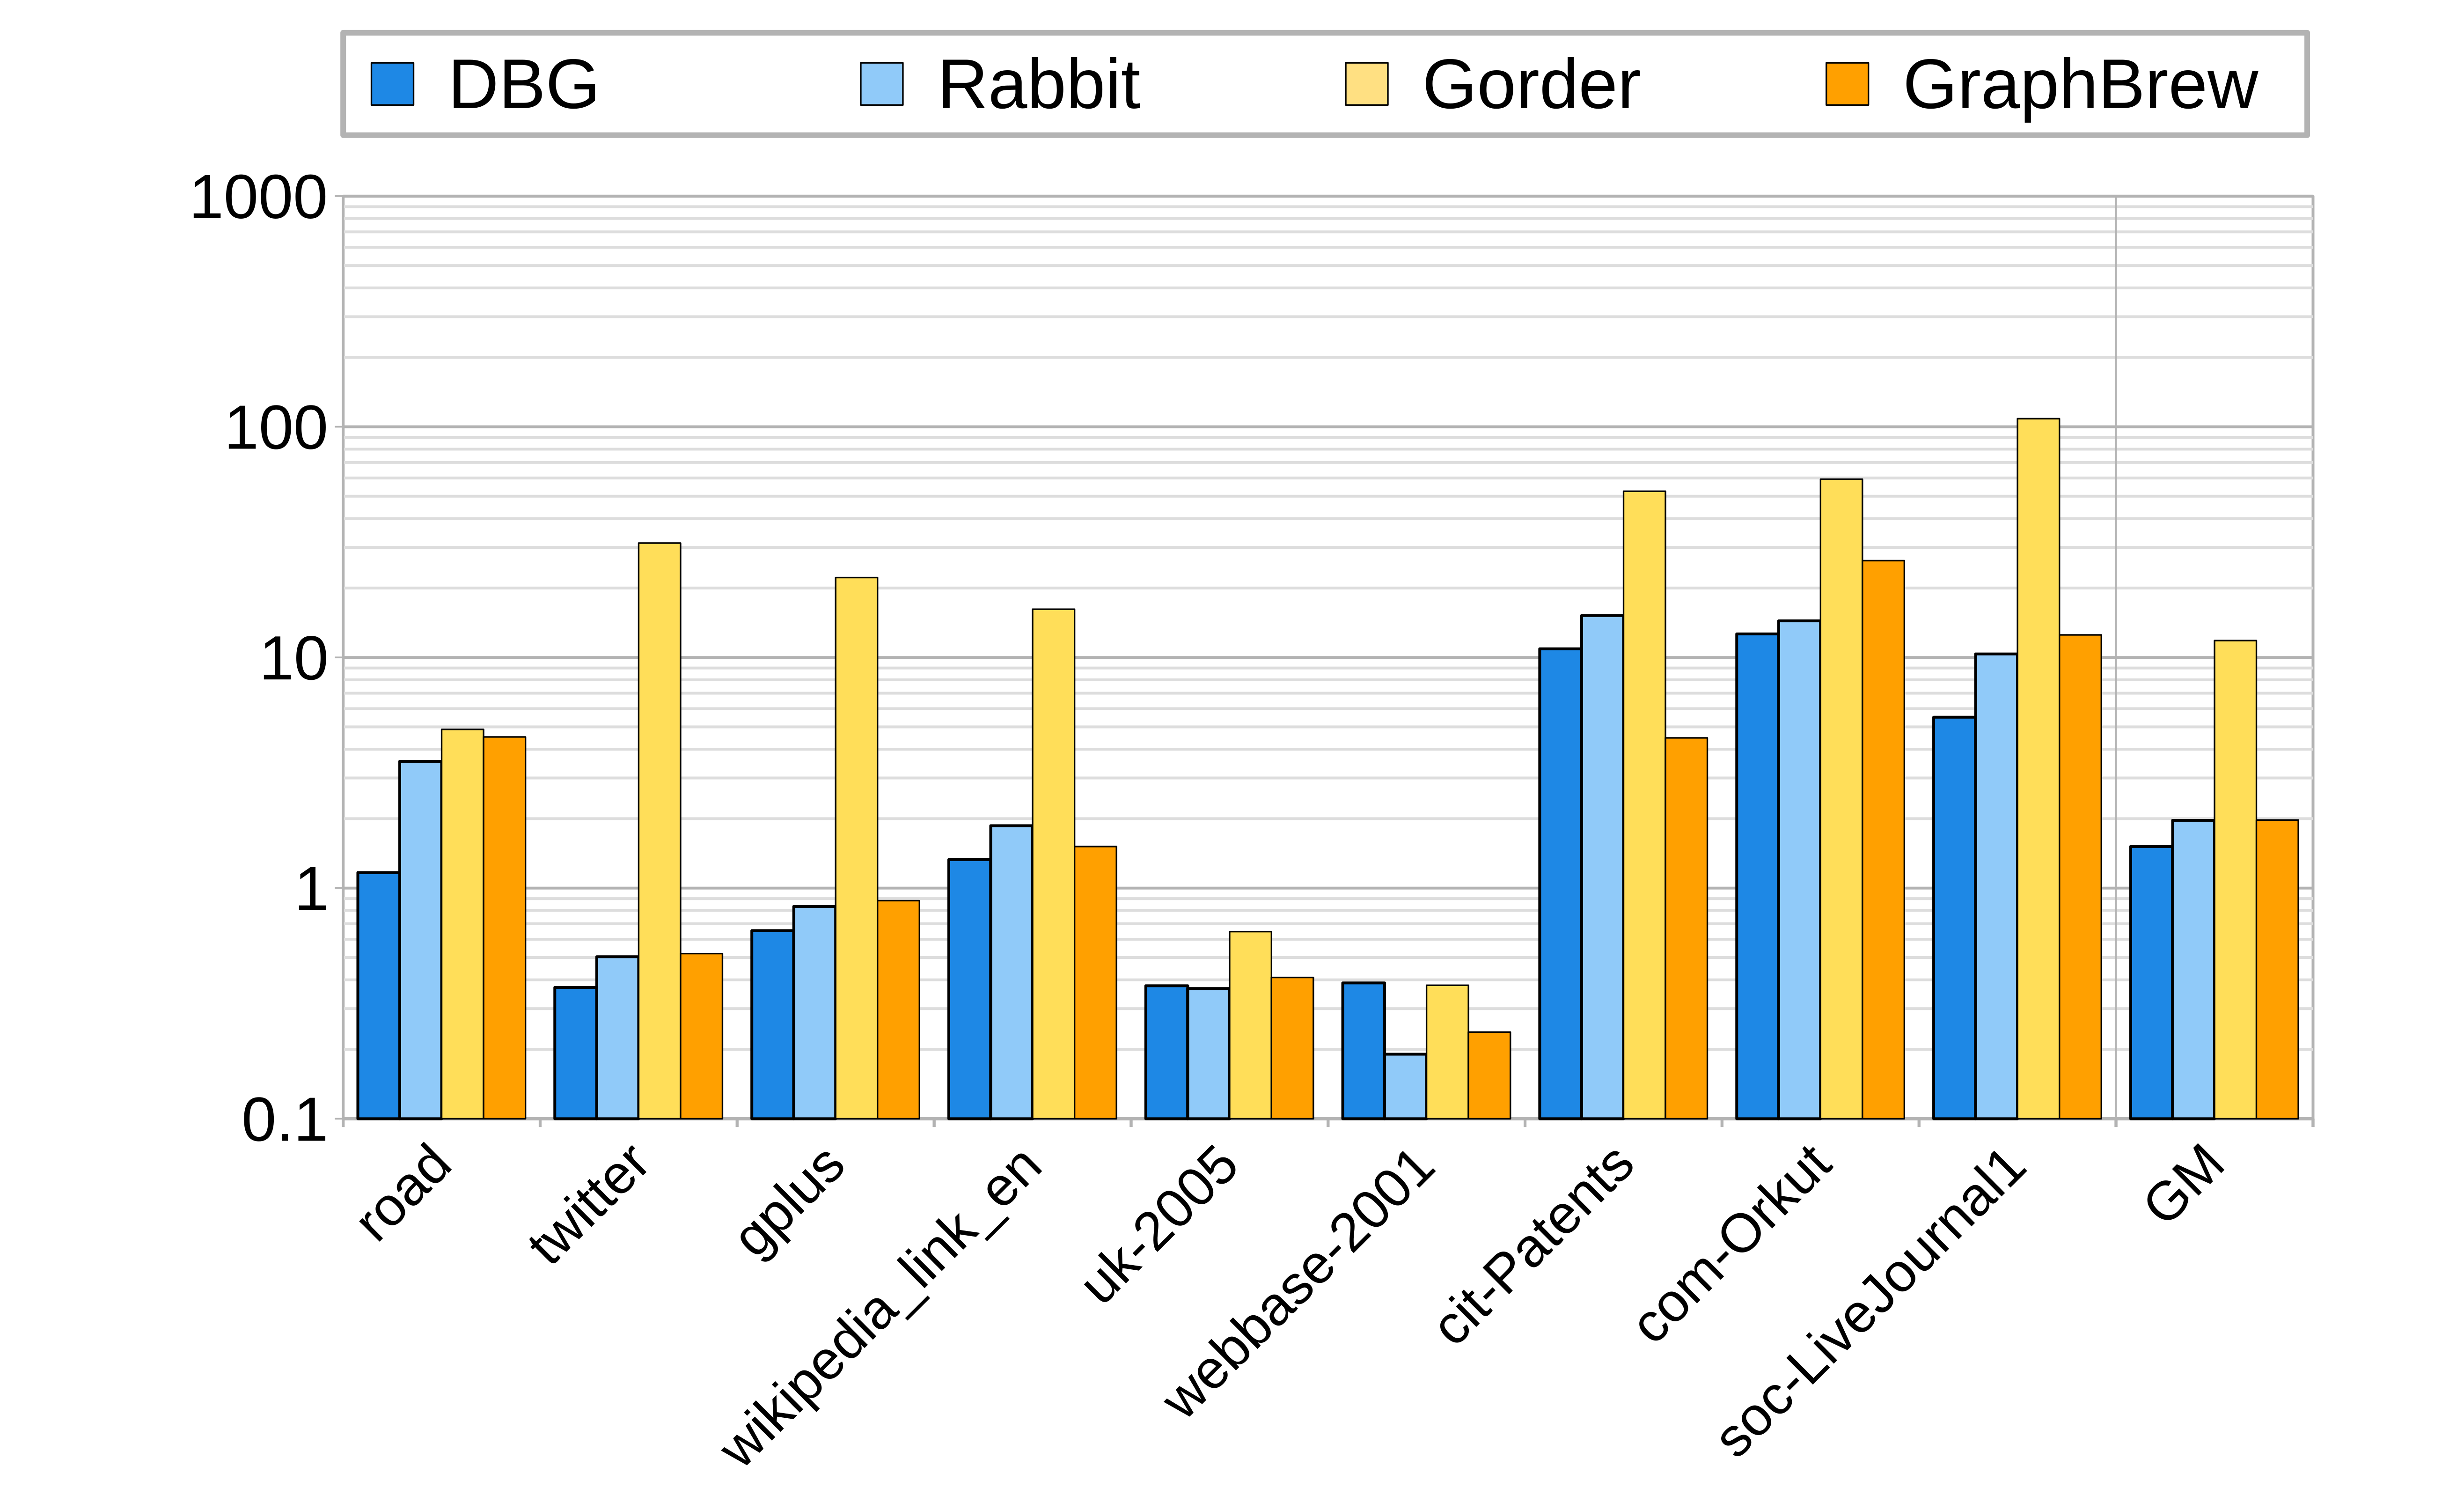
\includegraphics[width=\linewidth]{dataCharts/trials/SPMV}
\label{fig:trials:SPMV}
\end{subfigure}
\begin{subfigure}{.32\linewidth}
\caption{Connected Components (CC)}

\includegraphics[width=\linewidth]{dataCharts/trials/CC}
\label{fig:trials:CC}
\end{subfigure}
\begin{subfigure}{.32\linewidth}
\caption{Aggregated trials for graph data-sets }
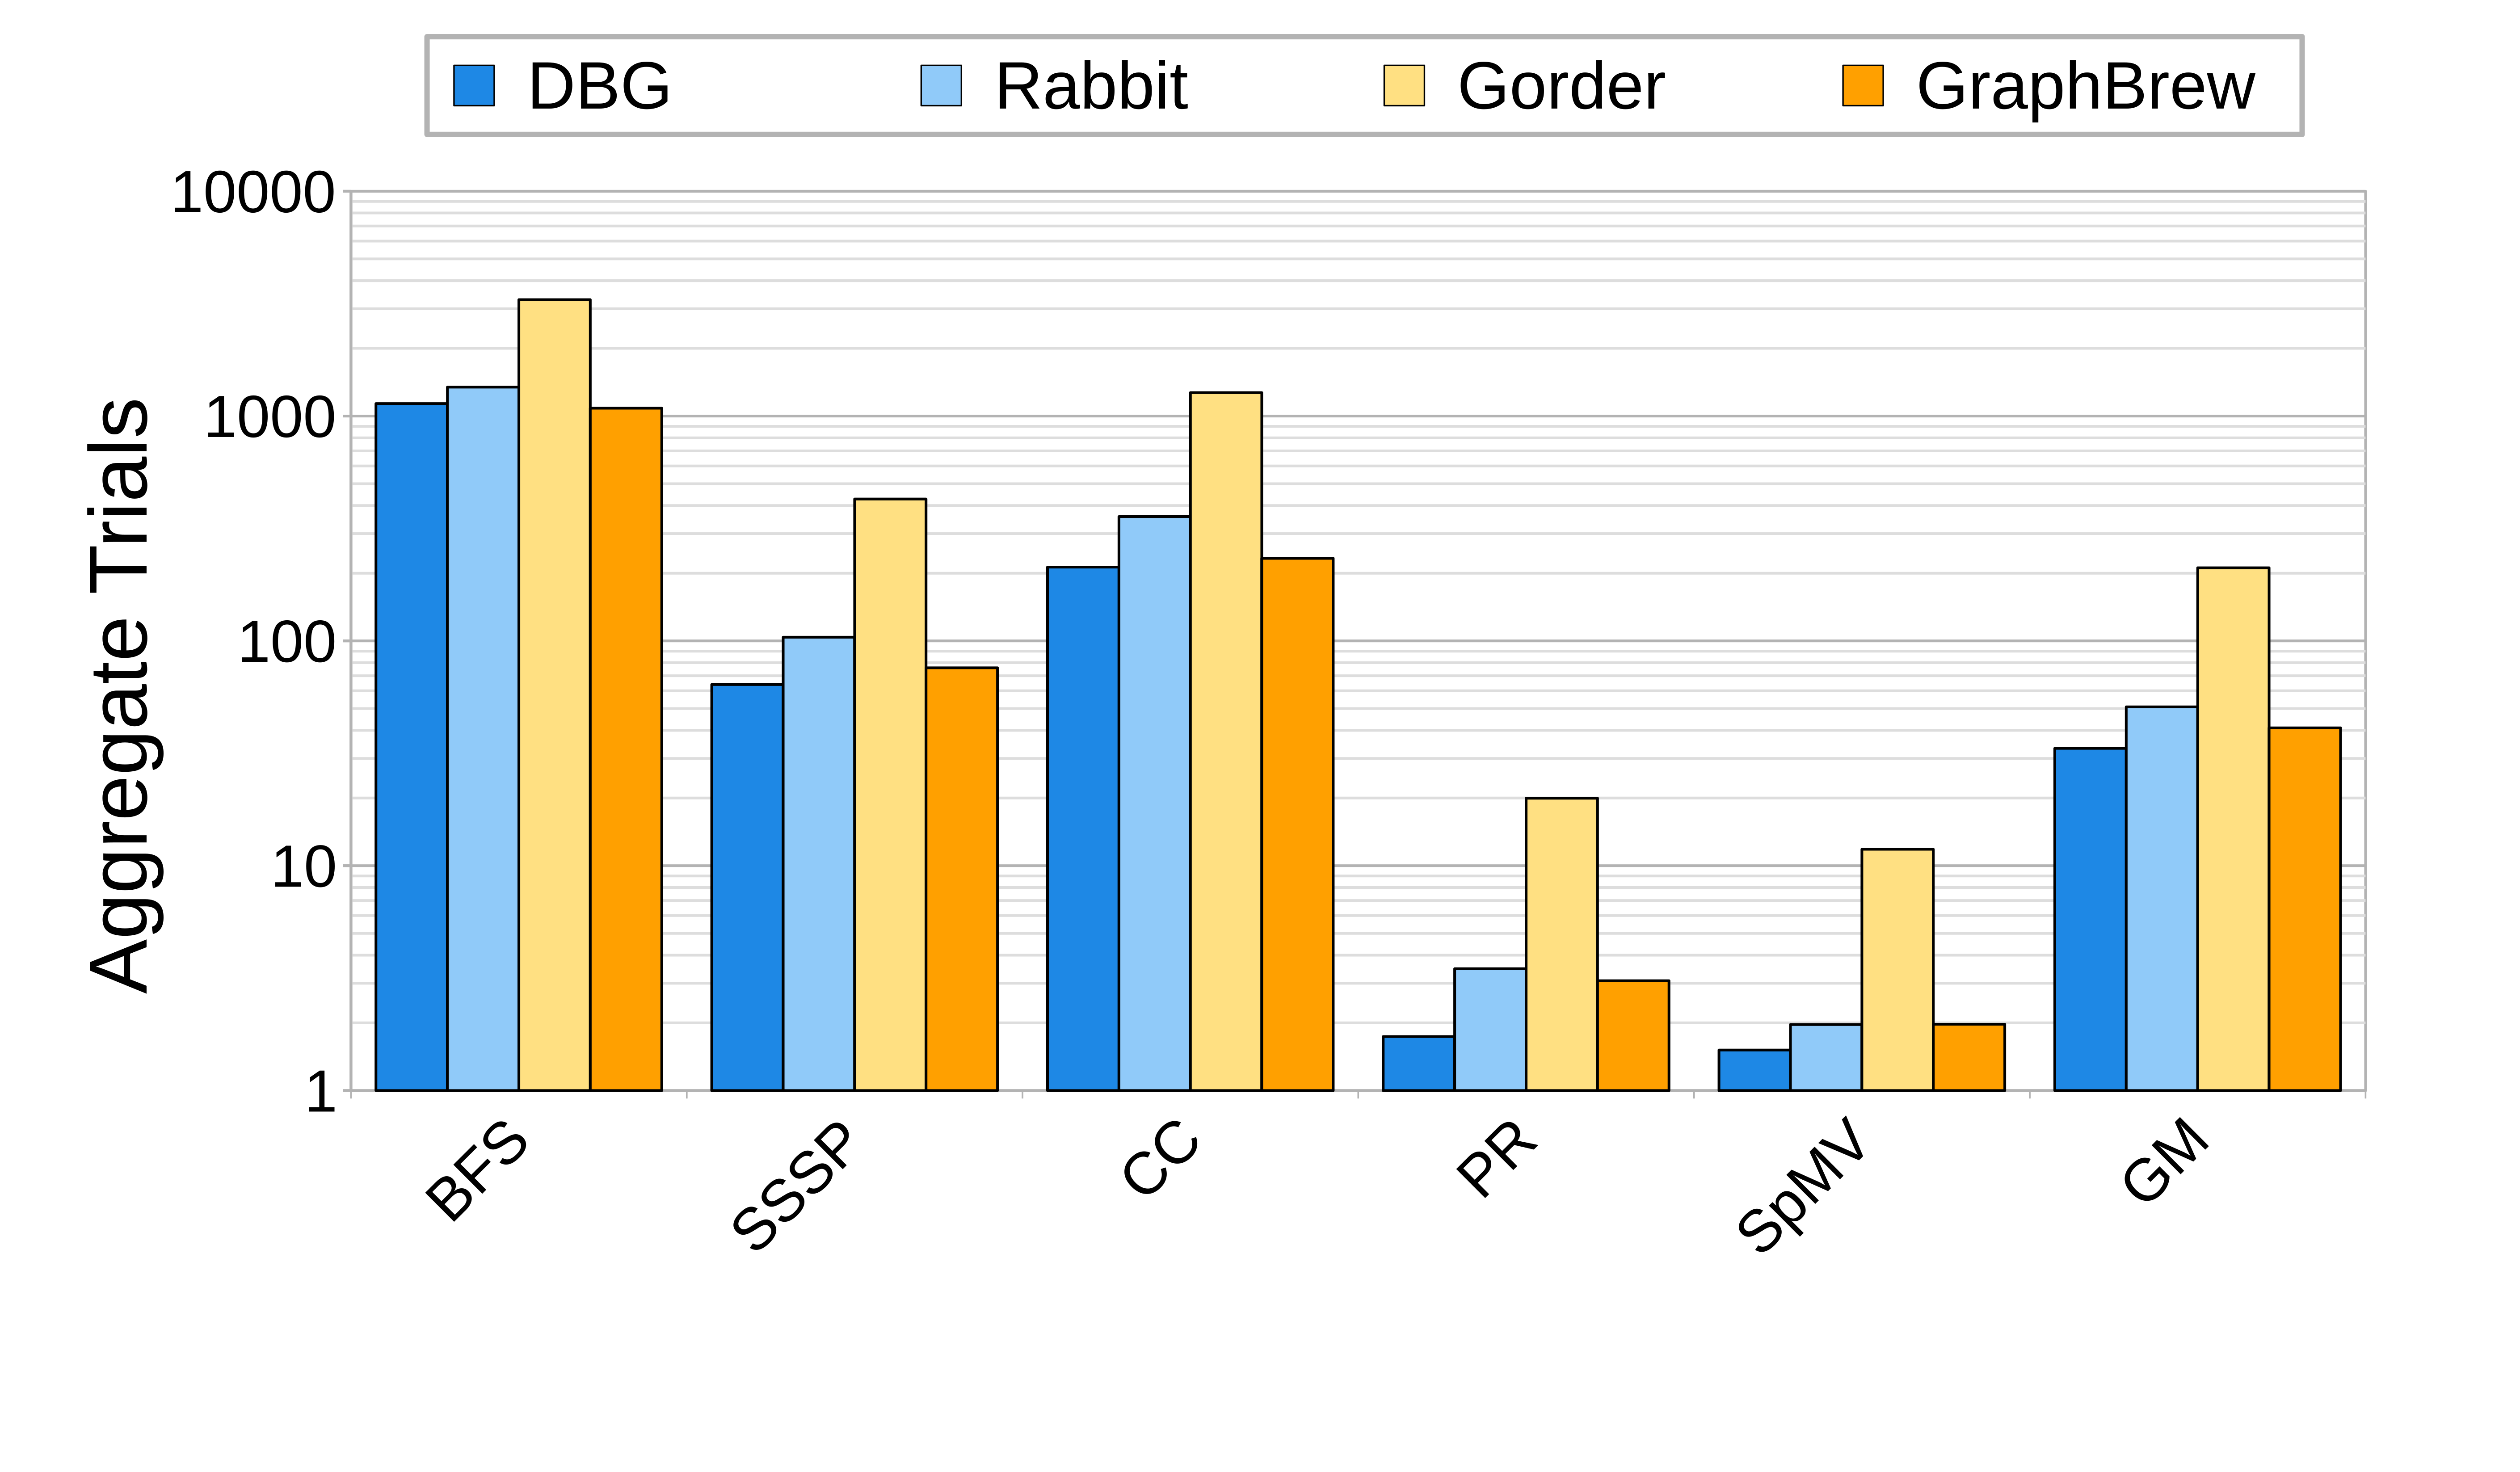
\includegraphics[width=\linewidth]{dataCharts/trials/aggregateTrials}
\label{fig:aggregateTrials}
\end{subfigure}

\caption{Trials needed to amortize reordering overhead. Comparison of GraphBrew lightweight reordering against other techniques -- Data are normalized to pre-processing with no reordering step.}
\label{fig:trials}
\end{figure*}

\begin{figure*}[ht]
\centering
\begin{subfigure}{.50\linewidth}
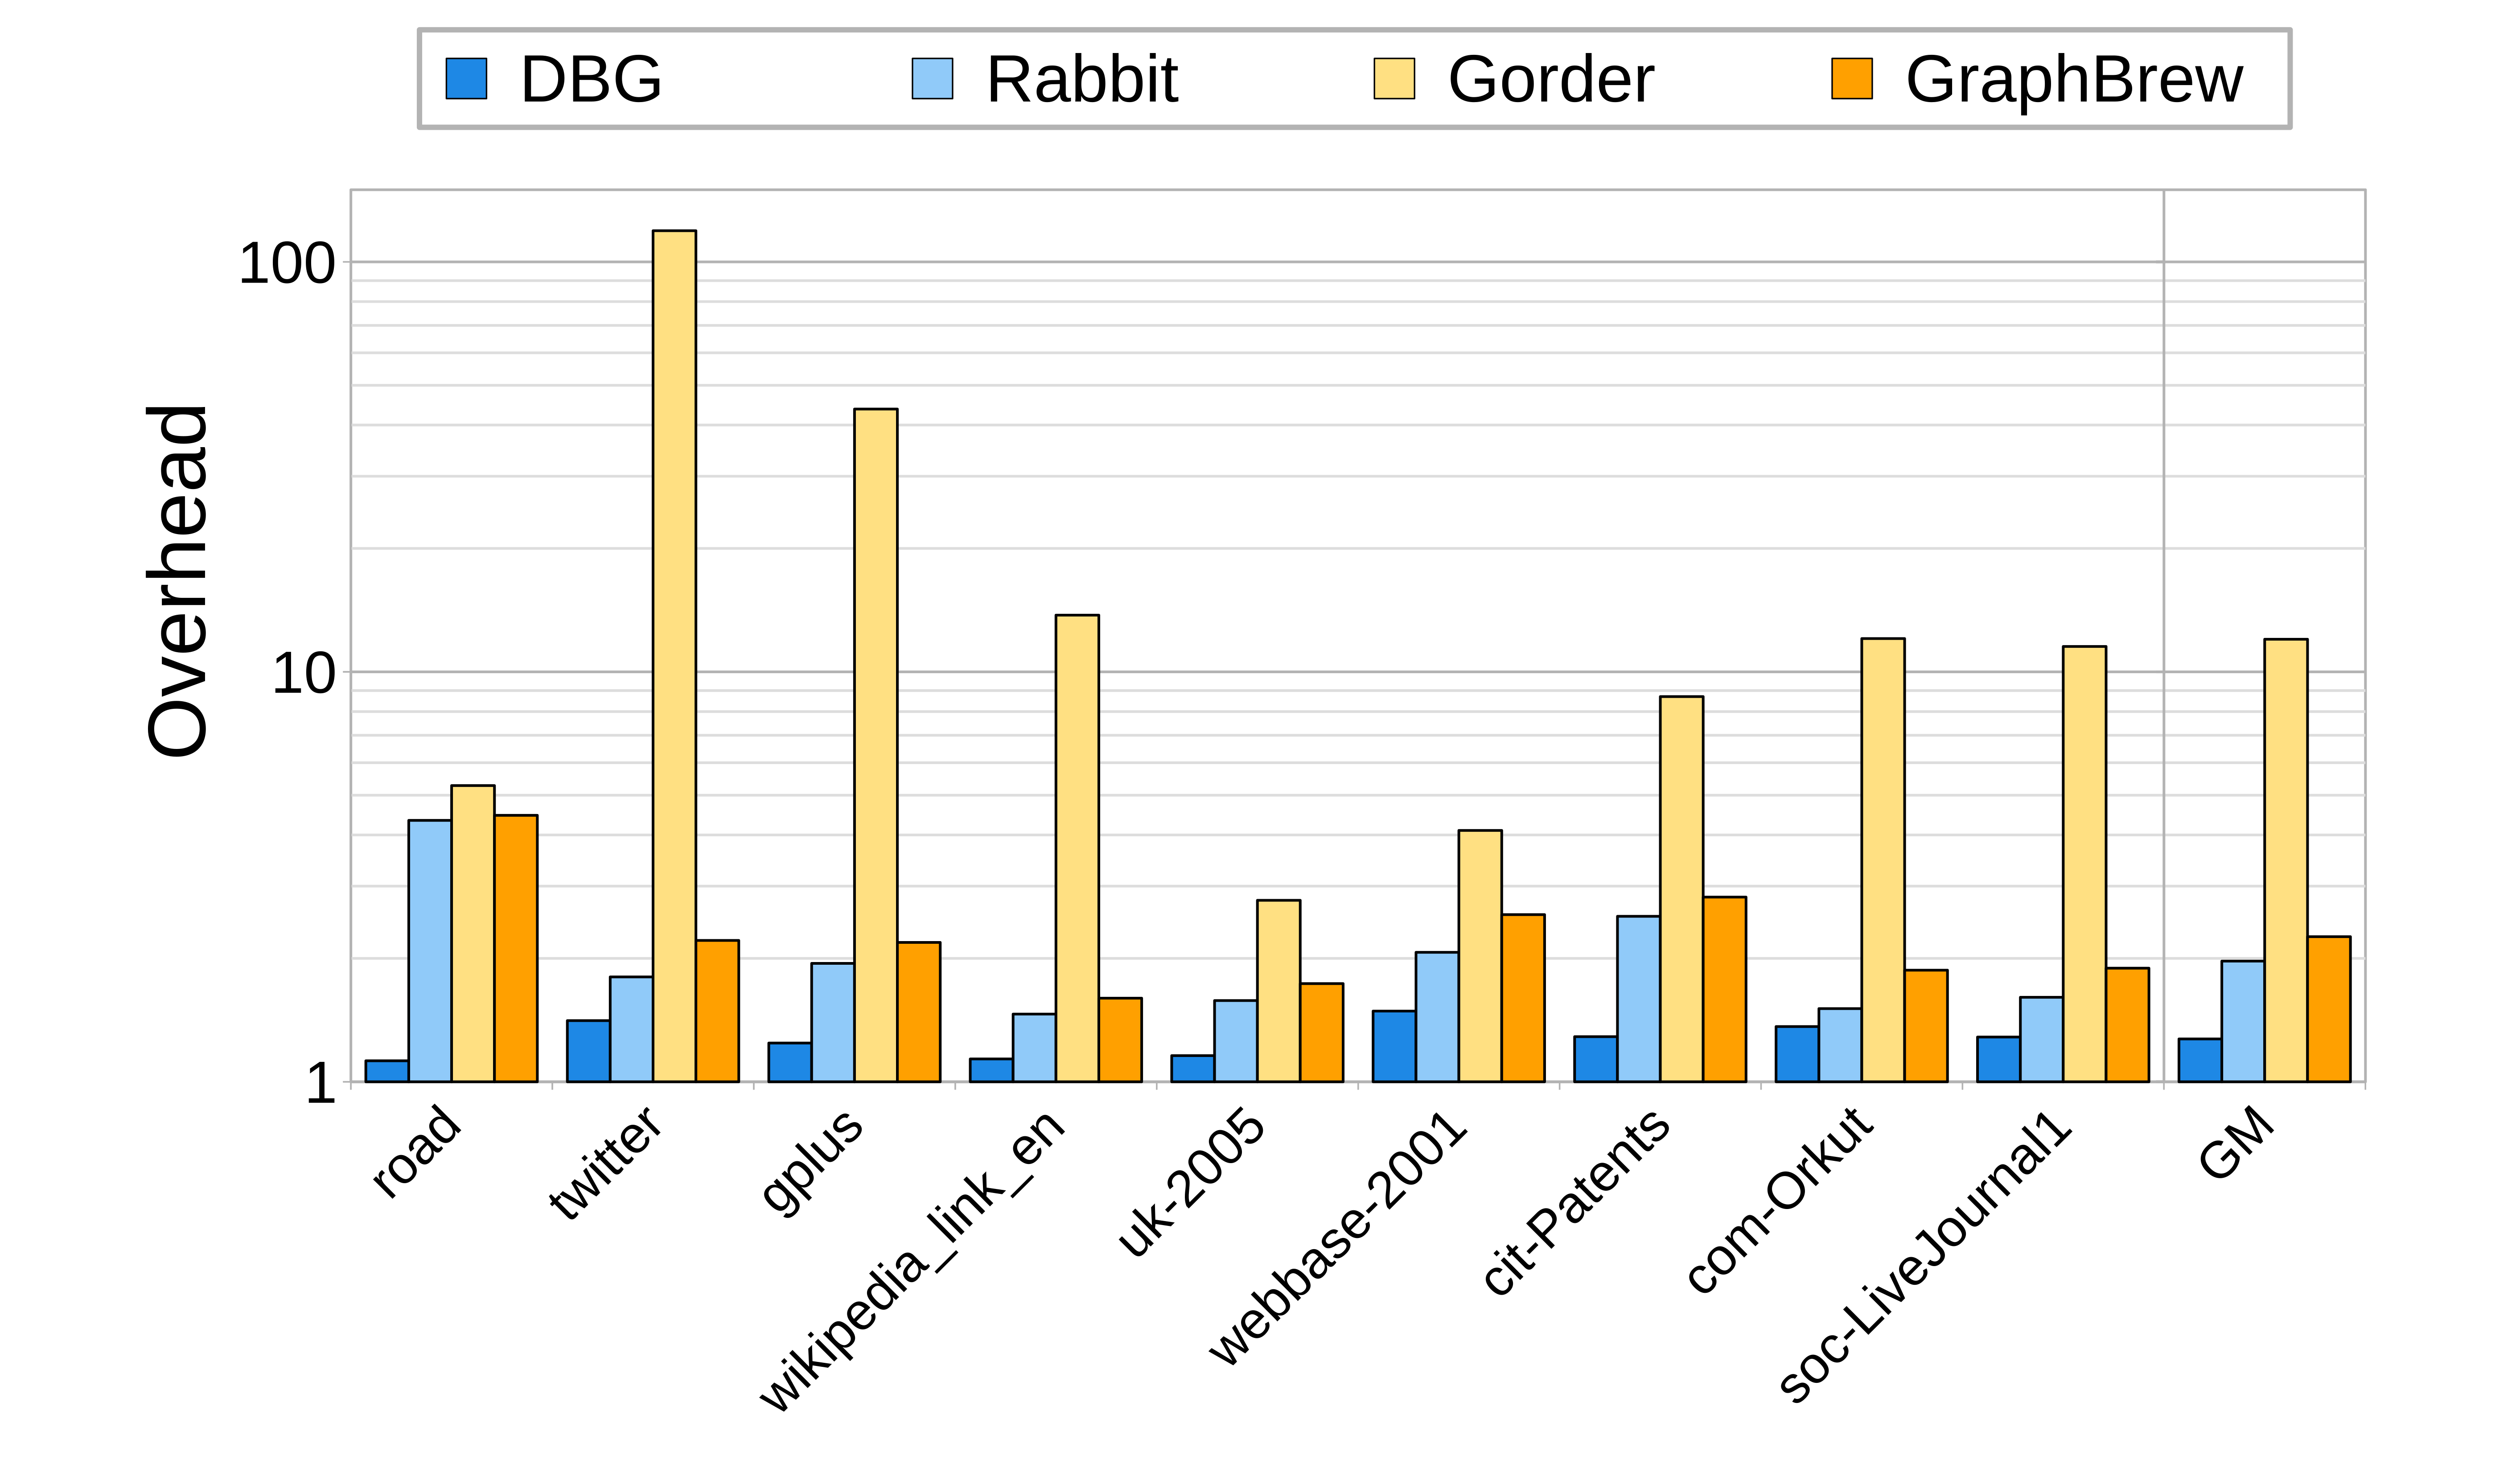
\includegraphics[width=\linewidth]{dataCharts/speedup/overheadReorder}
\label{fig:overheadReorder}
\end{subfigure}

\caption{Aggregated overhead comparison for GraphBrew lightweight reordering against other techniques -- Data are normalized to run-time with the original graph random labeling performance. Note how Graphbrew achieves better performance and lower overhead compared to Gorder.}
\label{fig:aggregateSpeedOverhead}
\end{figure*}
\subsection{Caching with GraphBrew}
First, we determine the effectiveness of each reordering technique by evaluating the cache performance utilizing the PageRank (PR) iterative algorithm and sweeping through several cache sizes and set associativity configurations. Fig.~\ref{fig:cache:performance} shows that increasing the cache size beyond \SI{16}{\mega\byte} improves performance in almost all reordering techniques, except for large data sets where the vertex data array caching performance is limited by the cache capacity and randomness of the graph vertex labels. For example, in Fig.~\ref{fig:cache:road} due to the mesh topology of Road, simple degree-based reordering is not sufficient to improve the caching performance. Ensuring an order that guarantees load balancing while processing these types of graphs is more critical. For large graphs, as shown in Fig.~\ref{fig:cache:twitter} where the memory footprint of the data arrays is larger than the cache. Reordering the graph according to its skewness (DBG) provides similar performance to the community-based rabbit order technique, where both are still not comparable to Gorder. Finally, studying Fig.~\ref{fig:cache:cacheGM}, where we showcase the geometric mean for all data sets caching, we showcase that GraphBrew gives a similar cache miss rate to Georder.

\subsection{Performance}
Fig.~\ref{fig:aggregateSpeedups} showcases GraphBrew achieving 1.68x speedup compared to Gorder's 1.71x performance when the geometric mean is taken for all graphs. This similar performance is for most graph algorithms except for BFS in Fig.~\ref{fig:speedups:BFS} due to Gorder having a preprocessing BFS step that optimizes for traversal scenarios. Furthermore, Gorder is a bit faster than GraphBrew in SpMV. However, these speedups are negligible because of the reordering overhead Gorder incurs, as shown in the next section.

\subsection{Reorder Overhead}
 Fig.~\ref{fig:trials} showcases the number of trials needed to amortize the reordering overhead such that it is worth including in the preprocessing step. GraphBrew shows a similar tradeoff compared to DBG and Rabbit Order. For instance, Gorder in  Fig.~\ref{fig:trials:PR} requires 20 trials of PageRank, each trial running 100 iterations to realize the benefits of reordering. Whereas GraphBrew requires 3 trials to compensate for the overhead. For  Fig.~\ref{fig:aggregateTrials}, while DBG might require less trials to amortize the reordering overhead, the algorithm iterations are slower than GraphBrew.

 Finally, Fig.~\ref{fig:aggregateSpeedOverhead} showcases the aggregate reordering overhead for each graph. This evaluation opted to show a total end-to-end performance as certain graph algorithm trials are too short compared to the preprocessing step. Instead, we chose a split analysis approach to focus on each step. In conclusion, GraphBrew maintains a lightweight reordering performance while delivering comparable performance to Gorder.
 

\section{Related Work}
As graph reordering became frequently used in other algorithms for performance optimization, several reordering schemes have been proposed \cite{petit_experiments_2004,boldi_webgraph_2003,barik_vertex_2020,frasca_numa-aware_2012,karypis_fast_1998,karantasis_parallelization_2014,cuthill_reducing_1969,wei_speedup_2016,broder_resemblance_1997, chierichetti_compressing_2009, lasalle_multi-threaded_2013, george_nested_1973,arai_rabbit_2016}. These schemes broadly differ in their objectives and measures used for reording. In this section, we review some of the most recent works from the high-performance computing research community.

The Minimum Linear Arrangement (MinLA) \cite{petit_experiments_2004} and MinLogA \cite{boldi_webgraph_2003} are examples of \textbf{gap-based schemes}. Here, a \emph{gap} measures the separation (due to reordering) between vertex ids that are connected by an edge. A net lower value of the gap is generally favored as it is a good indicator of preserving locality \cite{barik_vertex_2020}.

\textbf{BFS-based methods} \cite{frasca_numa-aware_2012,karypis_fast_1998,karantasis_parallelization_2014,cuthill_reducing_1969} are more lightweight than other schemes. However, they fail to capture detailed properties such as community structures, as BFS only captures connections between vertices. Hence, they offer modest locality improvements \cite{arai_rabbit_2016}.

Gorder \cite{wei_speedup_2016} is a \textbf{window-based scheme} and is the state-of-the-art method in terms of locality optimization \cite{barik_vertex_2020}. It uses a sliding window of a certain length and passes it over the graph's natural order, trying to maximize a \emph{Gscore}. Due to its sophisticated analysis approach, Gorder incurs large overheads, especially with dynamic graphs.

\textbf{Community-based reordering} \cite{broder_resemblance_1997, chierichetti_compressing_2009, lasalle_multi-threaded_2013, george_nested_1973} aims at identifying densely connected vertices and communities in a graph. In such schemes, the output communities are clusters with vertices more tightly connected with intra-cluster edges than to the rest of the graph. Standard community-based approaches fail to achieve high locality and fast reordering simultaneously \cite{arai_rabbit_2016}. Rabbit Order \cite{arai_rabbit_2016} achieves high locality by mapping a graph's hierarchical community structures to an architecture's cache hierarchy. It first generates the communities using a modularity optimization heuristic before generating the final vertex order \cite{barik_vertex_2020}.

Considerable research focuses on lightweight reordering \cite{balaji_when_2018,faldu_closer_2020,chen_workload_2021}. Incorporating simple graph features such as vertex degrees rather than an in-depth analysis using community-based or window-based reordering. \cite{chen_workload_2021} proposes Corder, a lightweight cache-aware reordering scheme that exploits the cache hierarchy of multicore systems and promotes workload balancing.

\section{Conclusion and Future Work}

In this paper, we demonstrated how specific lightweight reordering techniques fail to deliver comprehensive solutions for various graph problems and structures compared to a heavyweight approach such as Gorder. We then introduced GraphBrew, a lightweight reordering approach that infuses multiple graph features while employing a layered approach. Our evaluation shows the effectiveness of this organization, as it provides an end-to-end performance optimization and maintains a low reordering overhead. Moreover, GraphBrew experiences a cache and algorithm performance similar to that of heavy and sophisticated techniques.
 
Future directions include exploring further layered techniques to find more optimal ways to reorder graphs. We also plan to infuse the reordering information in the vertex data to explore a software/hardware co-design with real-time caching capabilities.
%\clearpage

%%%%%%% -- PAPER CONTENT ENDS -- %%%%%%%%

%\clearpage

\bibliographystyle{ACM-Reference-Format}
\bibliography{references_sync}

\end{document}
\endinput
